% !Mode:: "TeX:UTF-8"
% !TEX program  = xelatex

% \documentclass{cumcmthesis}
\documentclass[bwprint]{cumcmthesis} %去掉封面与编号页,电子版提交的时候使用。

\usepackage{graphicx} %use graph format
% \usepackage{epstopdf}
\usepackage[framemethod=TikZ]{mdframed}
\usepackage{url}   % 网页链接
\usepackage{csvsimple}   % 网页链接
\usepackage{subcaption} % 子标题
% \usepackage{multicols}
\title{穿越沙漠游戏的最佳决策}
\tihao{B}
\supervisor{ }

\begin{document}

 \maketitle
 \begin{abstract}
    
针对穿越沙漠游戏中的游戏目标,考虑天气是否全程已知、是否存在多玩家博弈等情形,分别建立模型,给出策略,并针对具体关卡进行求解。

在问题一中,全程天气状况已知。对沙漠地图进行抽象和简化,通过最短路算法计算关键路径,得到有向图。在此基础上,构建动态规划模型,使用记忆化搜索实现算法,求解给定初始状态下的最优策略。通过多重搜索算法,搜索所有的初始状态,从而得到指定关卡的全局最优策略。第一关和第二关的最优策略中,最终剩余资金分别为10470元和12730元。

在问题二中,由于环境存在不确定性,不确定性的累计效应会影响最终所做出的决策,因此我们建立了以关键结点为基础的简化模型,并以此建立了
用户的决策路径。
同时,为了保证玩家的收益以及最好应对不确定环境,玩家应该采取部分特定的策略,比如由于第二天仍然可以高温,所以在高温天气也应该照常行走。
最后,可以以剩余资金作为目标函数、时间和资源等为约束条件建立规划模型,建立参数之间的联系,从而分析用户应该采取的基本分析策略。
% 比如在资源或时间仅剩余一定量时应该前往终点、通过分析收益与成本关系来决定是否应该挖矿等。
基于此模型,对问题三四的关键结点位置的状态以及成本与收益进行分析后,即可获得最终的一般策略。

在问题三中,存在多玩家博弈。针对在起点处做出全部决策的情形,建立完全信息静态博弈模型。对地图进行简化后,用动态规划模型计算决策集合,得到赢得矩阵,求出2个纳什均衡。进而建立线性规划模型,求出混合策略。针对每一步都须做出决策且天气未知的情形,建立马尔可夫决策过程,引入风险接受程度,通过蒙特卡洛模拟分析风险接受程度对决策和最终剩余资金的影响,得出一般策略。


\keywords{动态规划 \quad 静态博弈\quad 马尔可夫决策 \quad 蒙特卡洛模拟}
\end{abstract}


\section{概述}
\subsection{问题背景}
\label{subsec:simulate}

在穿越沙漠游戏中,玩家凭借一张地图,利用初始资金购买一定数量的水和食物,从起点出发,在沙漠中行走。途中会遇到不同的天气,也可在矿山、村庄补充资金或资源,目标是在规定时间内到达终点,并保留尽可能多的资金。

在时间、资源和资金有限的情况下,需要考虑环境是否确定、玩家之间的博弈,针对不同的情况作出合理的决策,从而在保证不失败的情况下最大化游戏的收益。

针对环境是否确定,可分为全程天气状况已知、仅知道当天的天气状况两种情形,分别讨论两种情形下的最优策略和最佳策略。针对玩家之间的博弈,需要讨论多玩家博弈条件下玩家应采取何种策略。

本文将在考虑玩家可能会产生决策的关键节点的基础上,通过网络模型对地图进行简化后,讨论动态规划的决策过程、不确定状态下的阶段性决策路径、多玩家条件下的博弈,逐步解决该背景下的问题。

\subsection{目标任务}

问题一:在全程天气状况已知且只有一名玩家的条件下,对于给定的地图一定存在全局最优策略。考虑游戏规则,建立可推广到一般情况下的数学模型,并针对第一关和第二关求解出全局最优策略。

问题二:如何在环境不确定的状态下作出最优决策,使得利润最大化。考虑关键节点和不同决策阶段,建立决策路径,使得玩家在只知道当天天气的情况下,能够不失败并获得最大化。

问题三:如何在多人参加且决策会互相影响的情况下,预先作出策略或根据环境作出最优策略。考虑预先做出全部策略和动态做出策略两种情形,建立相应的决策模型,得出博弈的一般最佳策略。


\section{符号说明与模型基础}
\label{sec:simulate}

\subsection{符号说明}

本文所采用的模型如表\ref{tab:sign}所示,主要采用字母缩写下标模式命名,部分较少使用的变量在使用时定义。

\begin{table}[!htbp]
    \caption{本文符号}\label{tab:sign} \centering
    \begin{tabular}{p{1.5cm}p{3cm}|p{1.5cm}p{3cm}|p{1.5cm}p{3cm}}
        \toprule[1.5pt]
        符号 & 含义 & 符号 & 含义 & 符号 & 含义\\
        \midrule[1pt]
        $cost$ & 花费 & $m_{init}$ & 初始资金 & $w_{cost}$ & 水的基准价格 \\
        $cap_{basic}$ & 基础收益 & $c_{total}$ & 总计花费  & $f_{cost}$ & 食物的基准价格 \\
        $w_{sun}$ & 晴天基础耗水 & $w_{hot}$ & 高温基础耗水 & $w_{dust}$ & 沙暴基础耗水 \\
        $f_{sun}$ & 晴朗基础耗食物 & $f_{hot}$ & 高温基础耗食物 & $f_{dust}$ & 沙暴基础耗食物\\ 
        $m_{left}$ & 剩余的钱 & $f_{left}$ & 剩余的粮食 & $w_{left}$ & 剩余的水 \\
        $f_{buy}$ & 购买的粮食 & $w_{buy}$ & 购买的水 & $d_{total}$ & 总的天数 \\ 
        $d_{cur}$ & 当前天数 & $point$ & 玩家位置 & $k$ & 阶段数 \\
        $s$ & 状态 & $x$ & 决策 & $D$ & 决策集合 \\ 
        $d_{min}$ & 绕道矿山到终点 & $cap_{total}$ & 全部收益  & $cost_{total}$ & 全部花费   \\
        $c_{sun}$ & 晴朗基础消费 & $c_{hot}$ & 炎热基础消费  & $c_{dust}$ & 沙尘基础消费    \\
        \bottomrule[1.5pt]
    \end{tabular}
\end{table}



\subsection{网络模型简化}
\label{subsec:shortest}

在问题一和问题二中,只有一名玩家,不存在玩家之间的博弈问题。又因为沙漠中所有区域的天气相同,除了起点、终点、村庄、矿山
和关键决策节点以外的区域是等效的,玩家只需要重点关注起点、终点、村庄、矿山所在的区域及部分玩家可能会作出不同决策的关键
节点。同时,考虑到游戏目标,可以删去一些不影响计算最优解的路径。据此,可以对原始沙漠地图进行抽象和简化成一个\textbf{有向图}。
如下图所示,箭头上的数字代表了两个节点之间的最短距离,每个节点上玩家均可决定等待或前进。

\begin{figure}[!h]
    \centering
    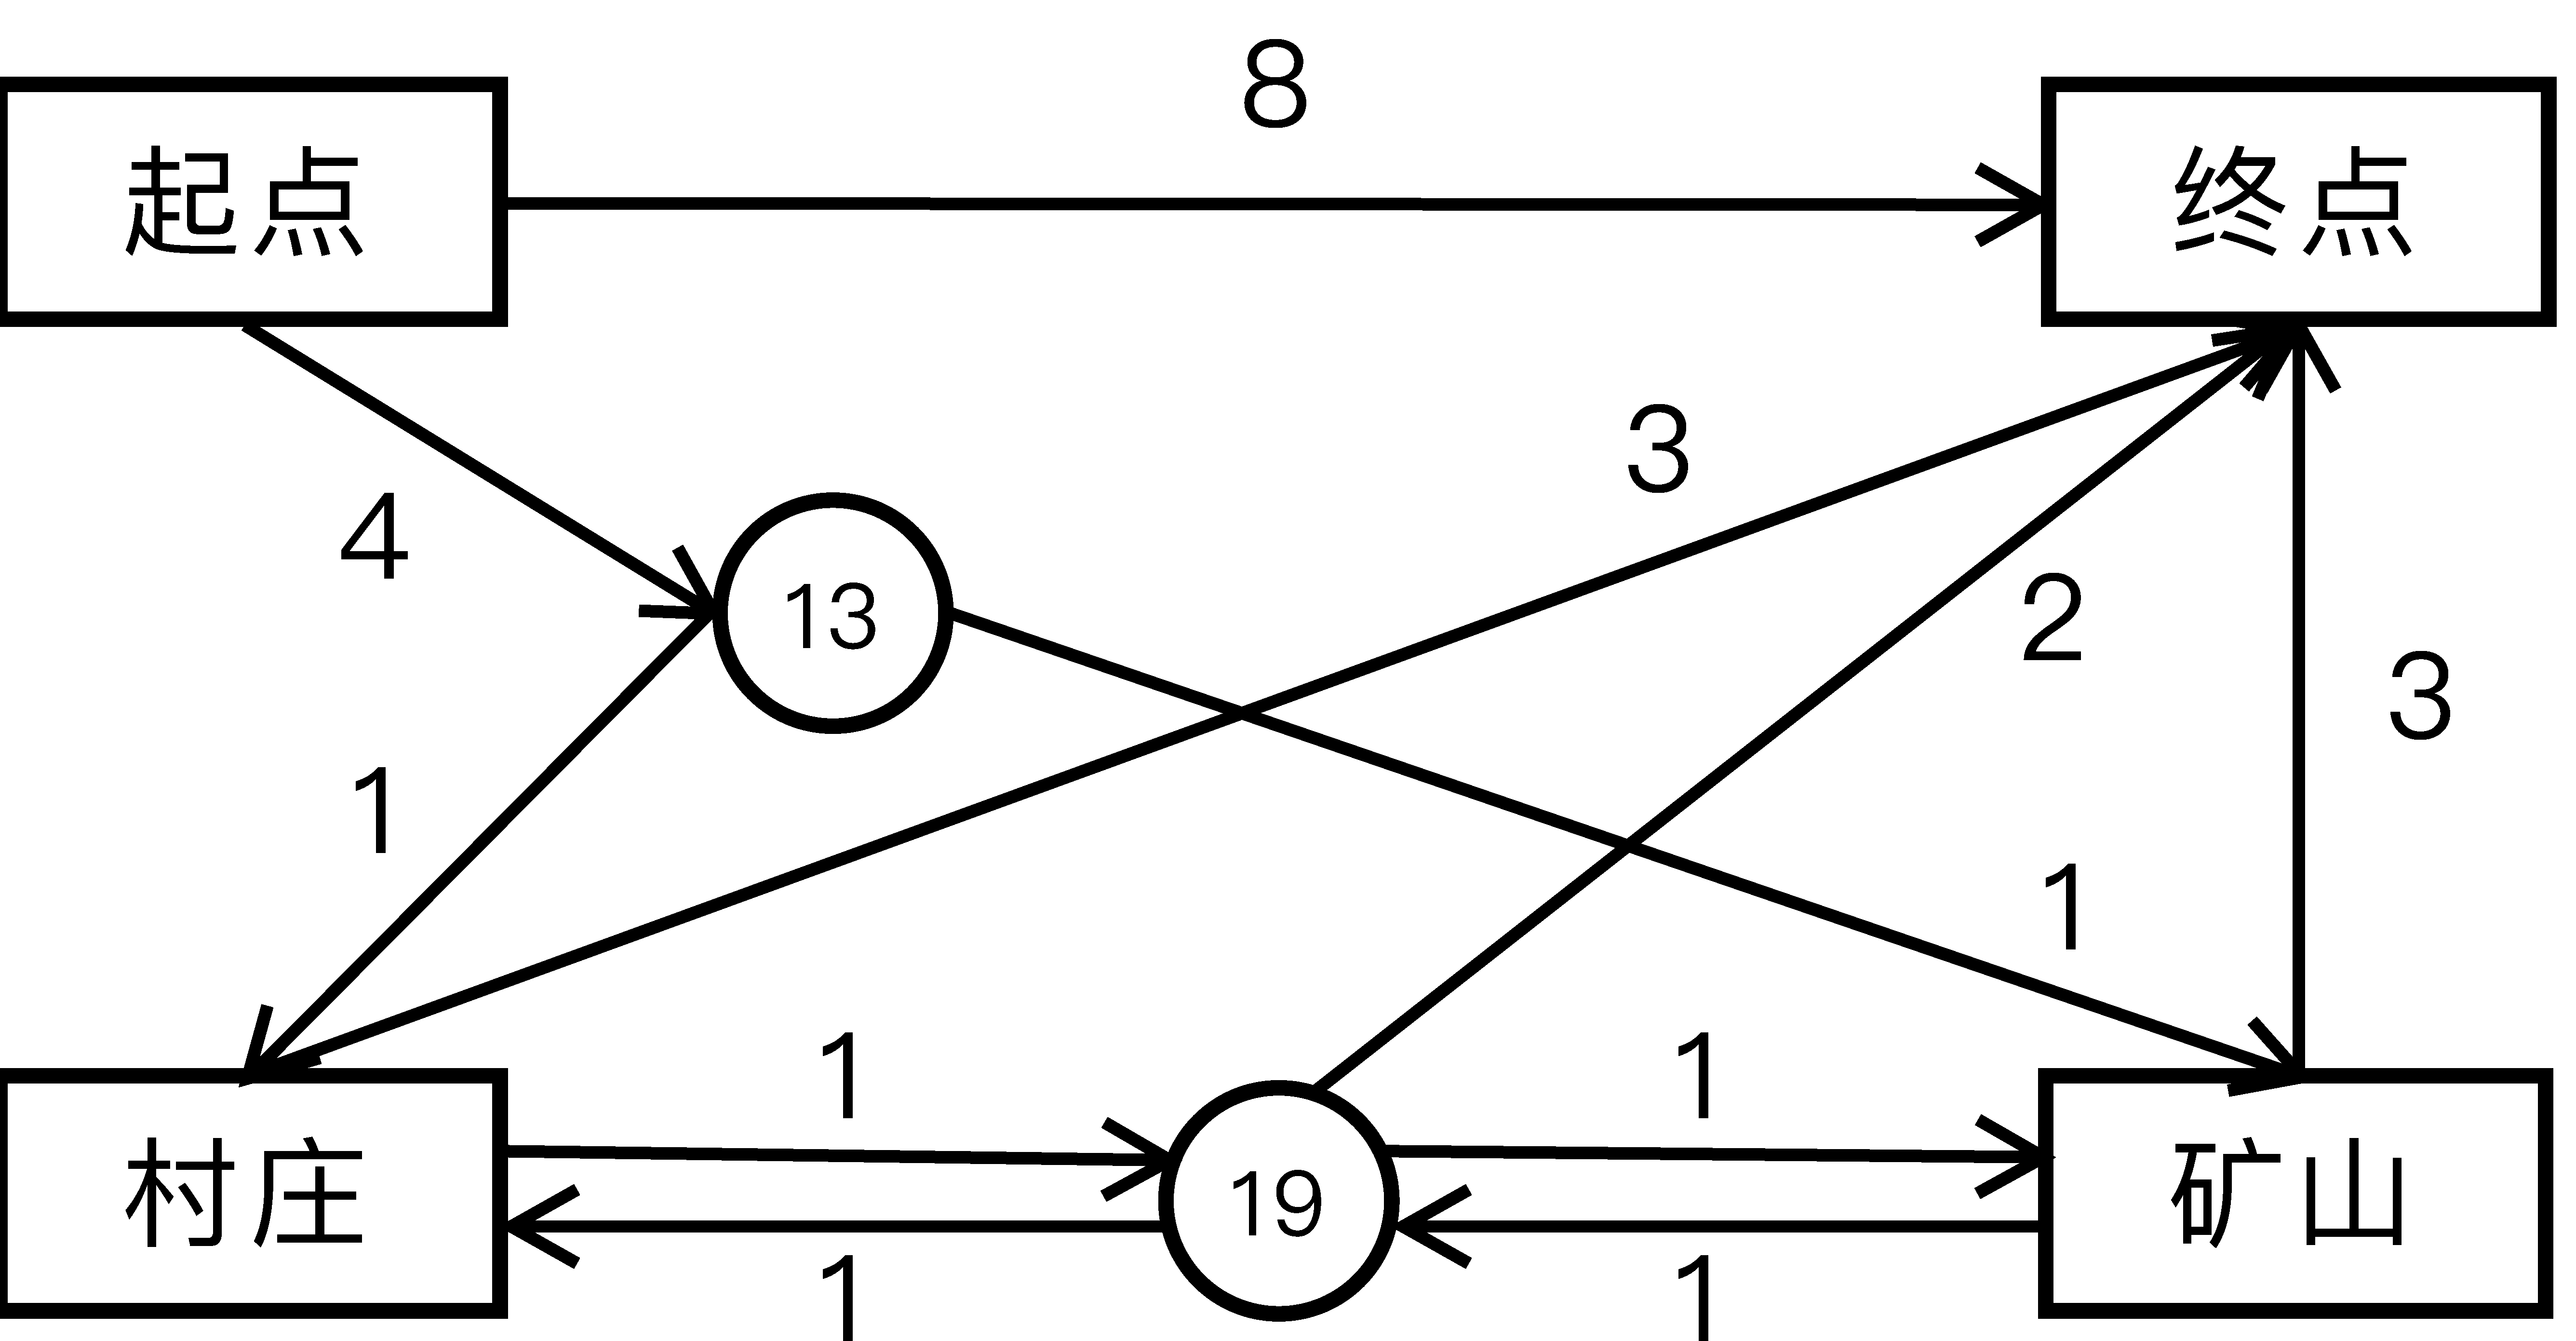
\includegraphics[width=.45\textwidth]{problem4-network}
    \caption{网络模型简化示意}
    \label{fig:problem4-network}
\end{figure}

在问题三/四中,由于状态是不确定的,所以存在路径决策的问题,点的效果是不等价的,需要寻找到累计状态最多的位置。
我们采用了调整后的Dijkstra算法与匹配算法对模型进行简化,获得点与点之间的全部路径后,通过匹配算法,根据实际情况计算路径中的重叠
位置,并选择部分节点作为关键节点。
比如第四关中,玩家可以到达13号节点再决定前往矿山还是村庄,13号是关键节点,第四关简化后的网络模型如图\ref{fig:problem4-network}所示。
具体算法请参考附录C。



% 最终可以建立出一个更为简单的模型,该模型只考虑关键节点,即玩家可能会作出的不同决策的位置。



\section{全程天气状况已知条件下的最优策略}
\label{sec:simulate}

\subsection{分析}
在本问题中,整个游戏时段内每天天气状况事先全部已知,且游戏的时间有限制,即游戏在有限步内结束。因此,玩家行动策略的总数是有限的,其中必然存在一个最优策略。对于策略总数有限的问题,可以通过穷举法找出其中的最优策略。然而,本问题中游戏策略众多,单纯使用穷举法的计算量过大。使用\textbf{动态规划}方法,将多阶段决策问题中的决策序列(整体策略)转化为若干子策略,可以有效减少计算量。

\subsection{模型建立}
\subsubsection{有向图模型}
根据\ref{subsec:shortest}小节所述的方法,本问题中第一关和第二关的地图可以分别简化为如图\ref{fig:problem1-2-network.pdf}所示的有向图。
\begin{figure}[!h]
    \centering
    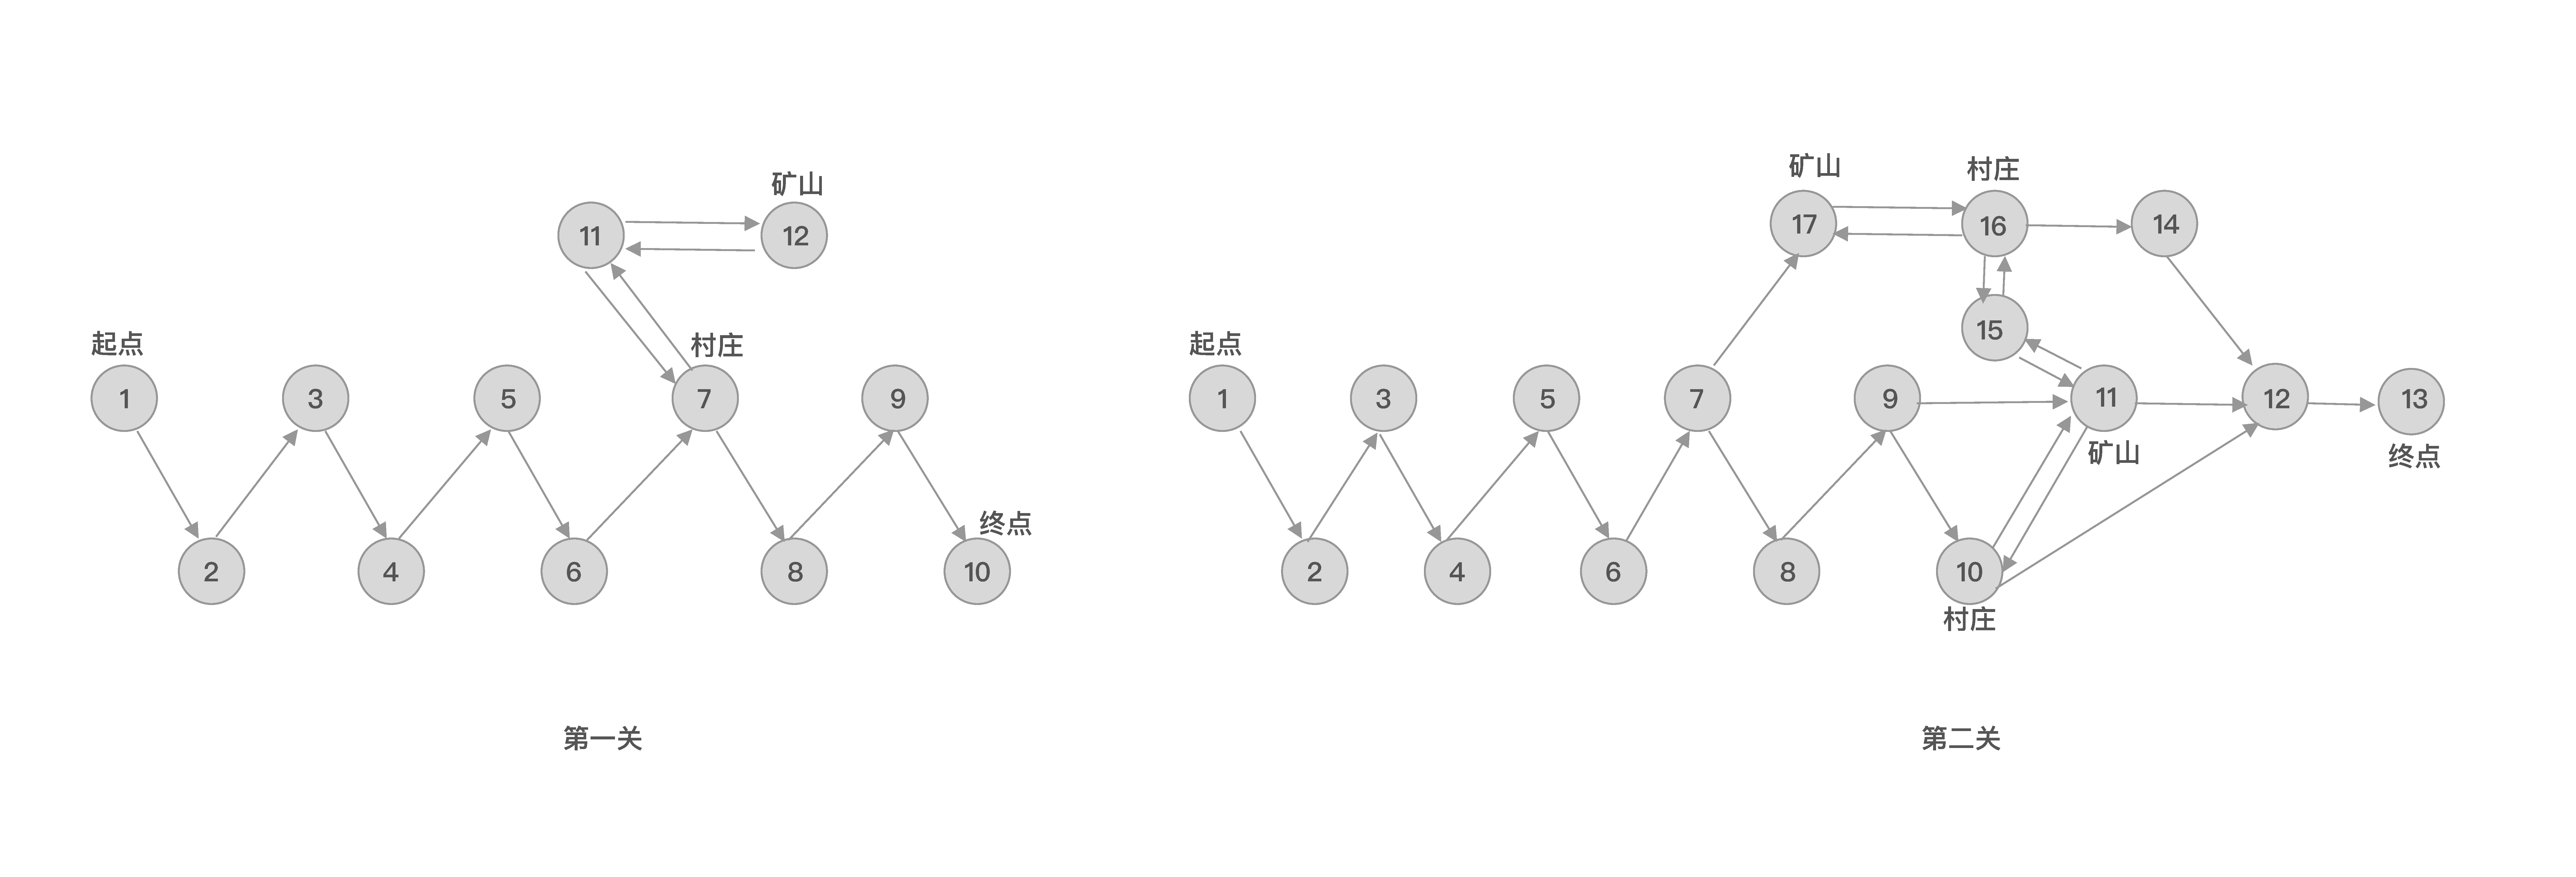
\includegraphics[width=\textwidth]{problem1&2-network.pdf}
    \caption{第一关,第二关:有向图模型}
    \label{fig:problem1-2-network.pdf}
\end{figure}

\subsubsection{动态规划模型}\label{dp}
\textbf{(1)阶段变量}

考虑到游戏规则中“以天为基本时间单位”,选取“天”为动态规划的分段依据,动态规划的阶段数与游戏中的当前天数相等,即
\begin{equation}
    k=d_{cur}
\end{equation}

\textbf{(2)状态变量} 

用$s_k$表示第$k$阶段的状态,其由玩家所处的位置、所携带资源(水和食物)的数量决定。
\begin{equation}
    s_k=g(point,w_{left},f_{left})
\end{equation}

$s_k$满足无后效性,即$s_k$一旦确定,从该阶段到游戏结束时的最佳策略(即从$s_k$出发的最佳子策略)不受第$k$阶段以前各阶段状态的影响。一旦各个阶段的状态都确定,整个游戏过程也就完全确定。

\textbf{(3)行为决策} 

用$x_k(s_k)$表示第$k$个阶段玩家处于$s_k$状态时的决策,$D_k(s_k)$表示第$k$阶段玩家处于$s_k$状态时允许的决策集合,故$x_k(s_k) \in D_k(s_k)$。根据游戏规则,可枚举出玩家处于不同状态时的决策集合。以第一关中玩家处于矿山(12号点)的状态为例,决策集合可表示如下:

\begin{table}[!htbp]
    \caption{第一关中玩家处于矿山时的决策集合}\label{tab:decisions} \centering
    \begin{tabular}{cccc|cccc}
        \toprule[1.5pt]
        决策编号 & 天气 & 路径 & 是否挖矿 & 决策编号 & 天气 & 路径 & 是否挖矿\\
        \midrule[1pt]
        $A_1$ & 晴朗 & 移动至11号点 & 否 & $E$ & 高温 & 停留 & 是\\
        $B$ & 晴朗 & 停留 & 是 & $F$ & 高温 & 停留 & 否\\
        $C$ & 晴朗 & 停留 & 否 & $G$ & 沙暴 & 停留 & 是\\
        $D_1$ & 高温 & 移动至11号点 & 否 & $H$ & 沙暴 & 停留 & 否 \\
        \bottomrule[1.5pt]
    \end{tabular}
\end{table}

在动态规划中,对于每一阶段、每一状态,可计算出具体的决策集合。

\textbf{(4)状态转移函数} 

每个阶段,玩家可能会发生资源和位置的变化,导致状态变化。状态转移函数如公式(\ref{state1})-(\ref{state2})所示。

\begin{equation}
    w_{left}=
    \begin{cases}
        w_{left}-n*w_{sun}& s_k \in \text{\{晴朗\}}\\
        w_{left}-n*w_{hot}& s_k \in \text{\{高温\}}
        \\
        w_{left}-w_{dust}& s_k \in \text{\{沙暴\}}
    \end{cases}
    \label{state1}
\end{equation}
\begin{equation}
    f_{left}=
    \begin{cases}
        f_{left}-n*f_{sun}& s_k \in \text{\{晴朗\}}\\
        f_{left}-n*f_{hot}& s_k \in \text{\{高温\}}
        \\
        f_{left}-f_{dust}& s_k \in \text{\{沙暴\}}
    \end{cases}
\end{equation}

\begin{equation}
    s_{k+1}=g(point_{k+1},w_{left},f_{left})
    \label{state2}
\end{equation}

在公式(\ref{state1})-(\ref{state2})中,
\begin{equation}
    n=
    \begin{cases}
        3 & s_k \in \text{\{挖矿\}}\\
        2 & s_k \in \text{\{移动\}}\\
        1 & s_k \in \text{\{停留\}} \cap \text{\{不挖矿\}}\\
    \end{cases}
\end{equation}

\textbf{(5)阶段损益函数} 

游戏的目标是在到达终点的前提下尽可能多保留资金,将资金的变化作为阶段损益函数。
\begin{equation}
    cost(s_k,x_k)=-p*w_{cost}*w_{buy}-p*f_{cost}*f_{buy}+q*cap_{basic}
\end{equation}
其中,
\begin{equation}
    p=
    \begin{cases}
        2 & s_k \in \text{\{补给\}} \& k \neq 0\\
        1 & k=0 \\
        0 & else
    \end{cases}
\end{equation}
\begin{equation}
    q=
    \begin{cases}
        1 & s_k \in \text{\{挖矿\}}\\
        0 & else
    \end{cases}
\end{equation}

基于以上说明,动态规划模型可总结为:
\begin{equation}
    \begin{cases}
        cost_{total}(s_0)=m_{init}-m_{left}(s_0) \\
        cost_{total}(s_{k+1})=cost(s_k,x_k)+cost_{total}(s_k) & k=0,1,2,...,d_{total}-1
    \end{cases}
\end{equation}
其中,$x_k \in D_k(s_k)$,$m_{left}(s_0)$为第0天补给后的剩余资金。

遍历最后一阶段中所有处于终点位置的状态,总计花费最少(剩余资金最多)的策略序列即为该初始状态下的最优策略。模型求解中,将考虑具体关卡的所有初始状态,以得到该关卡的全局最优策略。

\subsection{模型求解}
\subsubsection{算法简述}
由于在起点处(第0天)存在不同的物资补给策略,这些策略会影响初始状态,进而影响游戏过程中的决策序列和最终结果。因此,使用\textbf{多重搜索}算法分别考虑第0天水和食物的补给,对第0天的所有补给策略进行搜索,每种补给策略对应一个初始状态。确定初始状态后,使用动态规划模型计算出每种初始状态所对应的最优策略。最后,从所有初始状态所对应的最优策略中选出最优策略,即为关卡的全局最优策略。

在有村庄的地图中,村庄补给的策略过多大大增加了计算复杂度。因此,采用“先使用后记账”的策略对算法进行优化:允许资源存在缺口,每次经过村庄或到达终点时,若资源存在缺口,则检查缺口是否可在上一次经过村庄时得到满足。若可以满足,则补上缺口,扣除资金,保证了补给的最低限度;若无法满足(超过负重或上次经过村庄时资金不足),则进行\textbf{剪枝},停止此状态的继续递推。此外,考虑到模型的求解方向和状态转移函数的方向均为正向,求解过程中结合了\textbf{记忆化搜索}算法对经典动态规划算法加以改进。

算法使用Python进行实现,源代码见附录B。
\subsubsection{第一关}
通过多重搜索后,不同初始补给条件下最优策略的最终剩余资金如图\ref{p1_global}所示。图像底部$X$、$Y$坐标分别表示第0天购买的水和食物的数量,函数值为最终剩余资金。最终资金为0(深蓝色)的区域表示:这些初始补给条件下的资源数量超过负重上限或不足以支持玩家到达终点。
\begin{figure}
    \centering
    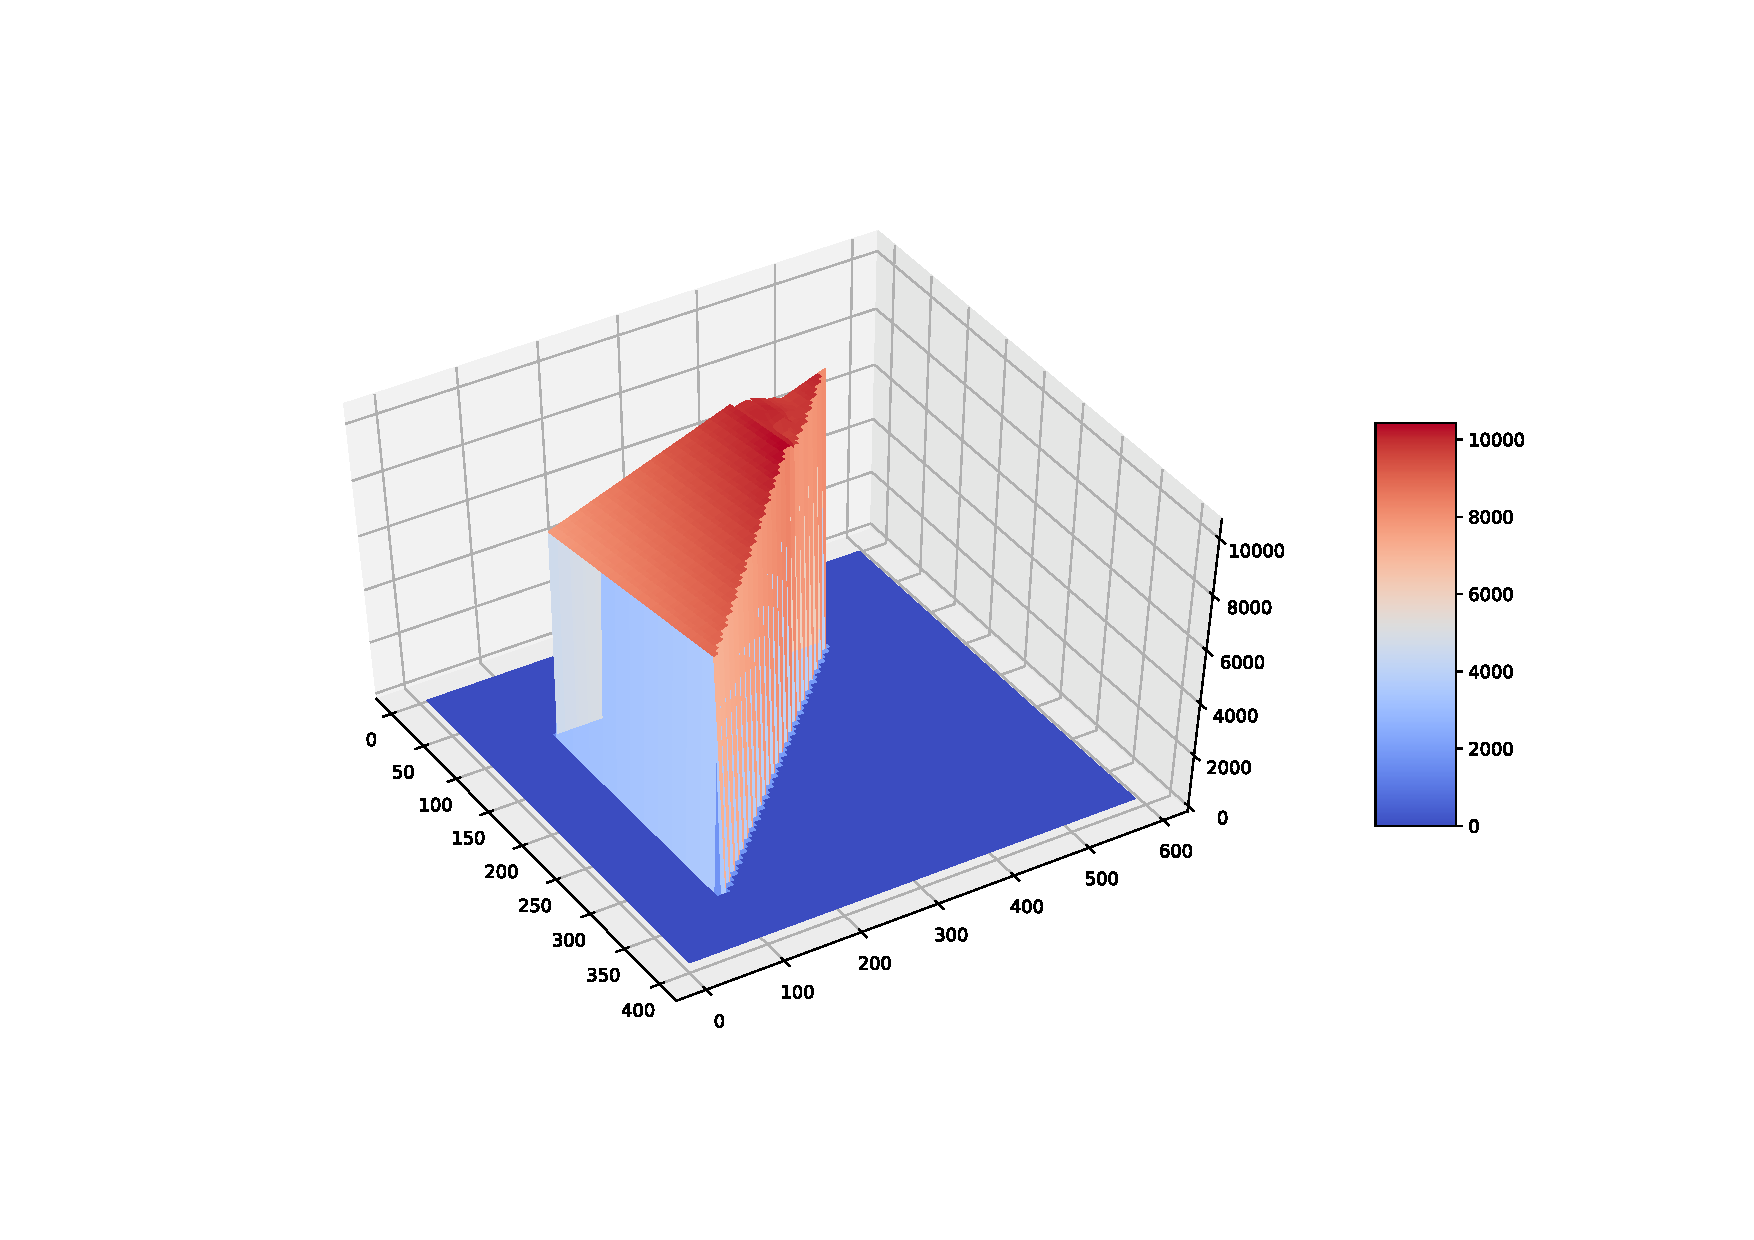
\includegraphics[width=8cm]{p1_global}
    \caption{第一关:不同初始补给条件下最优策略的最终剩余资金}
    \label{p1_global}
\end{figure}

经计算,第一关的最优策略为:第0天携带178箱水和333箱食物出发;第8天到达村庄并补给163箱水;第10天到达矿山,第11至19天在矿山停留,其中第11、17天不挖矿,其他日期挖矿;第21天再次到达村庄并补给36箱水和16箱食物;第24天到达终点,水和食物均刚好用尽;最终剩余资金10470元。详细计算结果见附录。
\subsubsection{第二关}
具体求解过程与第一关类似,不再赘述。经计算,第二关的最优策略为:第0天携带130箱水和405箱食物出发;第10天到达位于点16(原始地图中区域39)的村庄并补给10箱水;第11天停留在该村庄并补给179箱水;第12天到达位于点17(原始地图中区域30)的矿山;第13至18天在该矿山挖矿;第19天到达位于点16的村庄并补给196箱水和86箱食物;第21天到达位于点11(原始地图中区域55)的矿山;第22至28天在该矿山挖矿;第30天到达终点,水和食物均刚好用尽;最终剩余资金12730元。详细计算结果见附录。

\begin{figure}
    \centering
    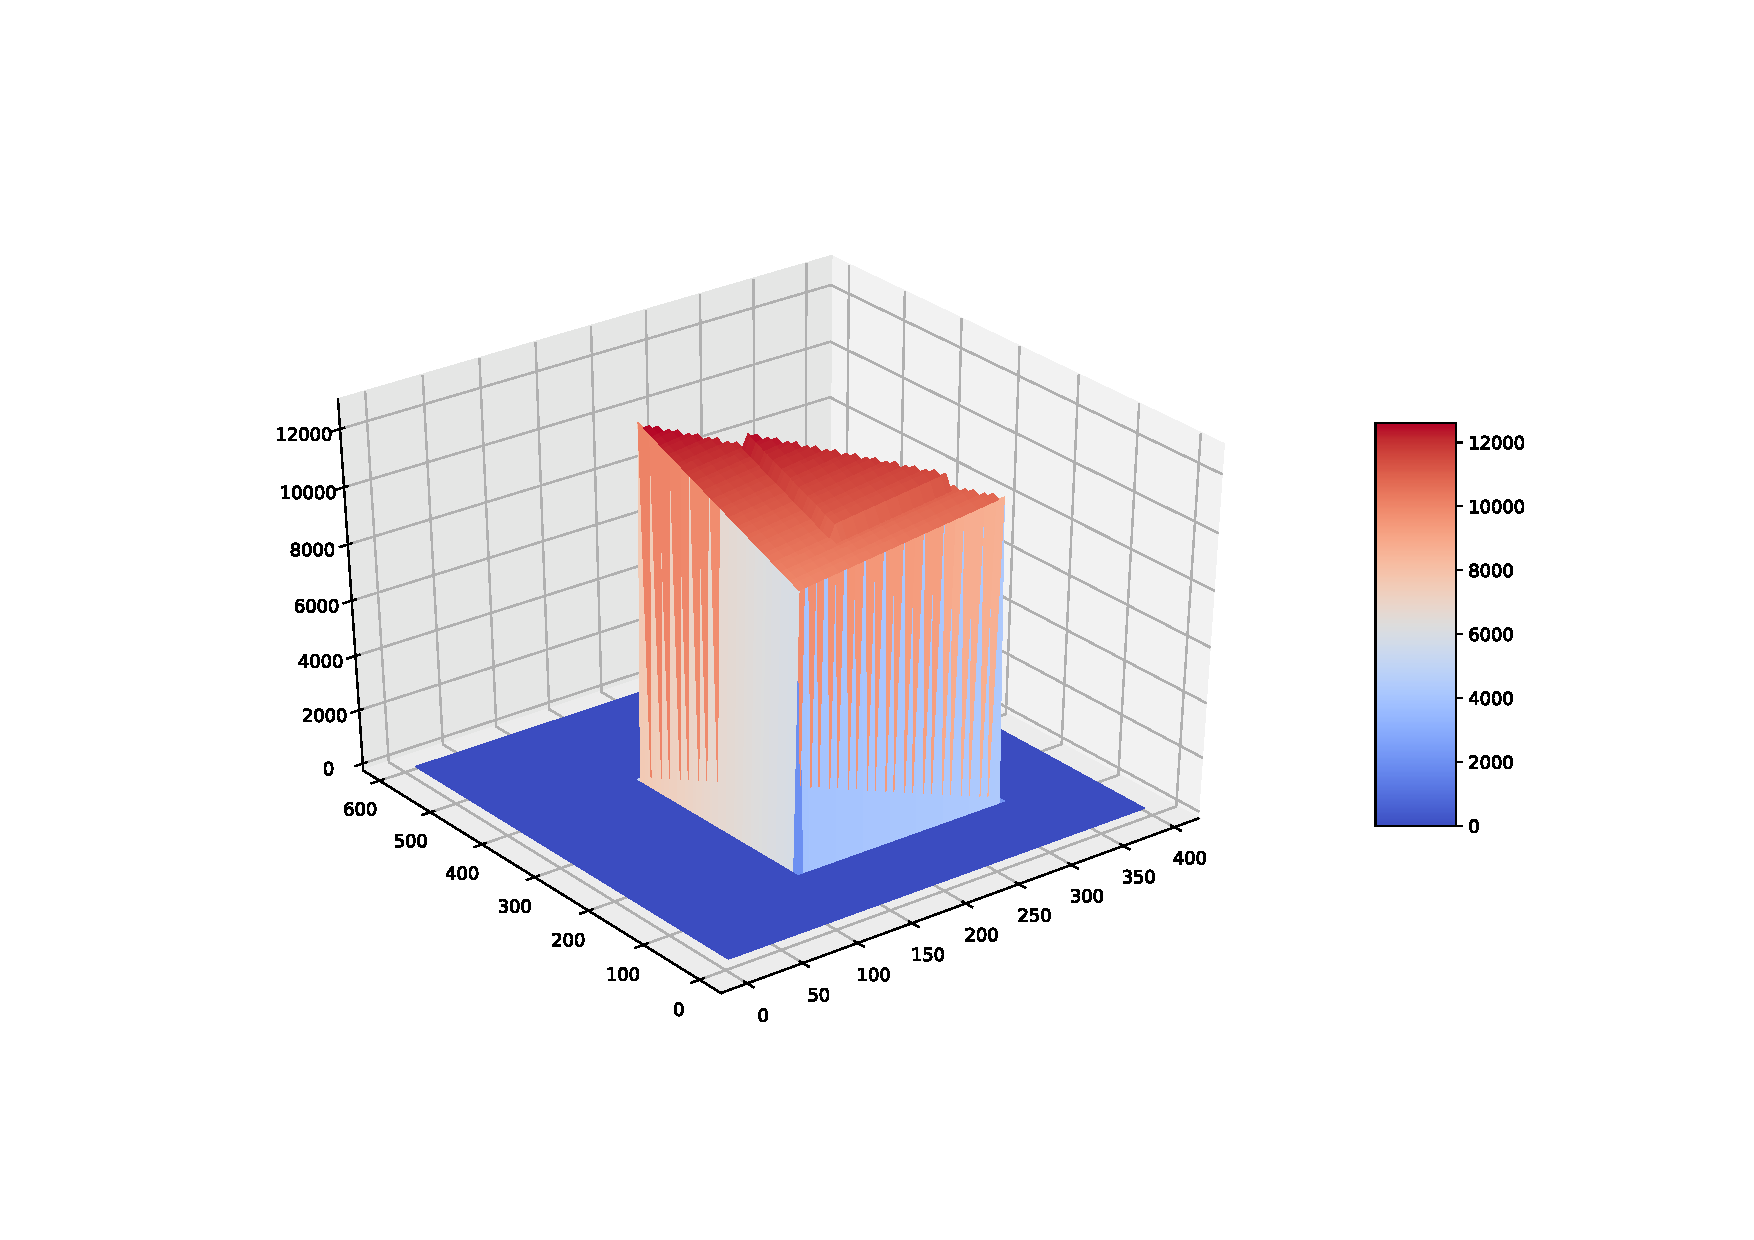
\includegraphics[width=8cm]{p2_global}
    \caption{第二关:不同初始补给条件下最优策略的最终剩余资金}
    \label{p2_global}
\end{figure}

\section{天气未知情况下一般的最佳策略}
\label{sec:simulate}

\subsection{问题分析}

在仅仅知道当天天气的情况下,玩家的最佳策略的主要约束条件是 :在保证游戏不失败的前提下,最大化游戏收益。
为了不保证游戏失败,玩家必须在指定的的时间内到达终点,同时保证仍然有水和食物剩余,这就需要玩家合理安排购买的物品以及在矿
山开矿的时间。

影响决策的最主要的因素是沙尘暴天气和炎热天气的比例,以及是否有村庄。
沙尘暴天气的出现概率小于100\%,否则玩家将无法前进;
炎热天气的概率为0\%-100\%,即可能一路上全部是炎热,也可能全部是晴朗;
村庄可能有,也可能没有;
矿山在该问题中预设是存在的,否则不需要研究如何最大化利益。


% \begin{table}[!htbp]
%     \caption{影响因素情况}\label{tab:001} \centering
%     \begin{tabular}{c|cccc}
%         \toprule[1.5pt]
%         影响因素 & 沙尘暴天气 & 炎热天气 & 村庄 \\
%         \midrule[1pt]
%         变量范围 & 0\%-99\% & 0\%-100\% & 有/无 \\
%         \bottomrule[1.5pt]
%     \end{tabular}
% \end{table}


% 以上的因素都会影响最佳决策的设计,比如如果没有村庄,则只需要考虑如何能够最优化在矿山的收益,以及如何
% 安全地到达终点,其决策路径必定是“起点$\to$前往矿山$\to$挖矿/休息$\to$终点”,或者直接“起点$\to$
% 终点”。
我们接下来将对模型进行简化,然后对决策因素的影响进行分析,考虑在部分因素不确定的情况下、部分因素确定的情
况下,一般玩家的最优决策。

\subsection{模型建立}

% 该模型的建立基于两个预设条件:
% (1)玩家能够在起点购买物品后,一次性到达终点。
% (2)玩家从起点到终点所需要花费的最小时间,略小于总的允许时间。
% 我们可以基于这两个假设条件,先对网络模型进行简化,将问题简化为决策路径确定情况下,如何最优化资源利用
% 效率的问题。

\subsubsection{网络模型简化}
\label{subsub:simplify}

根据\ref{subsec:shortest}的推导与附录A的算法,我们可以将网络进行预先简化为只有关键节点的模型。
以第四关为例,玩家需要从起点前往“矿山”或“终点”,为了实现最优策略,避免走路造成更多的消耗,途中必然会
选择最短路径,途中的大部分位置是等价的。
但是在13/19位置,玩家可以决定是先前往矿山还是村庄、是继续挖矿还是前往终点,这也是关键节点。

% 最短路径中会存在交集,比如前往矿山和村庄的最短路径中可以在13位置相交、村庄和矿山到终点的最短路径在19
% 号位置相交,在13/19号位置可能会产生决策行为,即是先前往矿山还是村庄、是继续挖矿还是前往终点。
% 根据\ref{subsec:shortest}小节的证明,我们可以通过最短路径算法,将路径简化为:

\begin{figure}[!h]
    \centering
    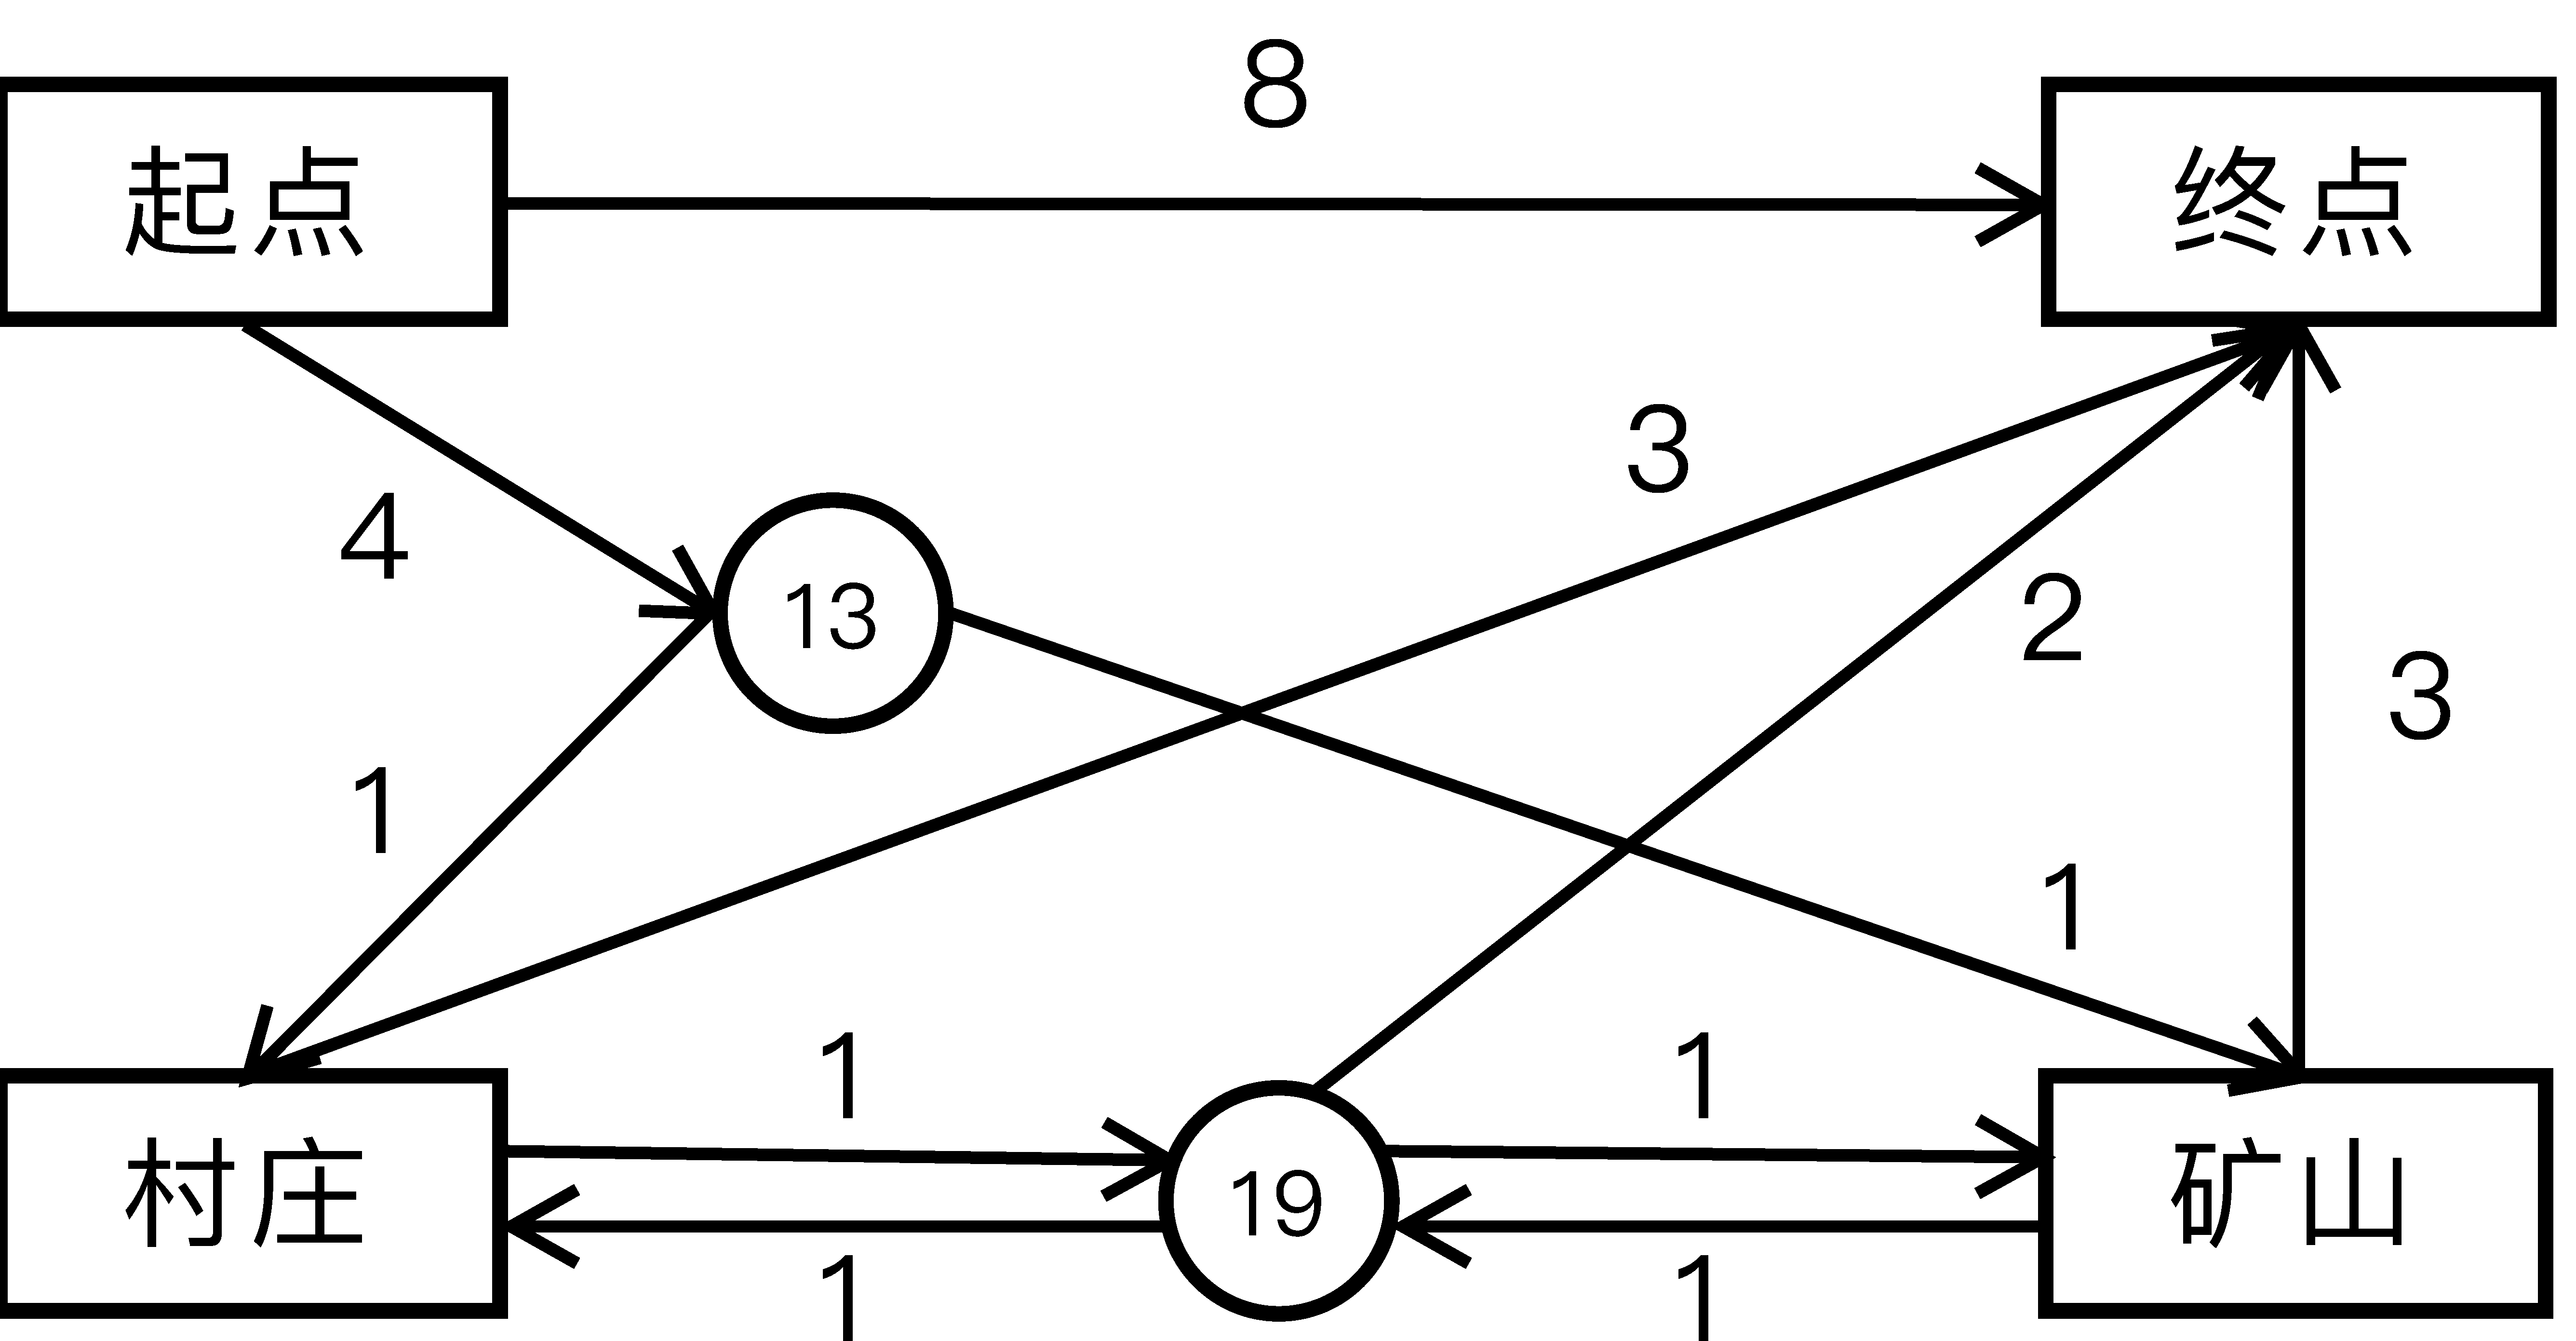
\includegraphics[width=.5\textwidth]{problem4-network}
    \caption{第四关-模型简化}
    \label{fig:example-network}
\end{figure}

在该图中,箭头上的数字代表两个地点之间需要行走的区块,在这些区块中玩家可以选择行走或停在原地。
同时,玩家到达“矿山”后可以选择停下不工作或“挖矿”。
由于玩家重新回到“起点”无法购买,而前往“终点”游戏结束,所以不存在从“矿山”前往“起点”或“终点”前往其
他位置的直线。


% \uline{在这个模型中,虽然我们没有考虑是否应该选择矿山和终点的中间路径,然后根据遇到的天气决
% 定是否前往矿山或终点,但是后续我们会说明,该简化方式不会影响我们的最优策略分析。}

\subsubsection{决策路径建立}

建立好简化版的网络模型后,我们可以建立玩家的一般决策路径,包括决策的各个阶段和各自的触发条件,然后
再量化比较不同路径的效果,从而得出最优策略。
\uwave{决策路径一般分为两个方向:(1)直接前往终点,包含直接终止阶段(2)绕行前往矿山后再前往终点,
包含初始阶段、挖矿阶段和终止阶段。}

% 同样以第四关为例,根据\cref{subsub:simplify}介绍的简化模型,我们可以将其转化为下述的决策过程:

\begin{figure}[!h]
    \centering
    
\includegraphics[width=.85\textwidth]{problem4-decision}
    \caption{第四关-决策路径}
    \label{fig:example-decision}
\end{figure}

同样以第四关为例,图\ref{fig:example-decision}是图\ref{fig:example-network}简化后的决策模型,
玩家可以选择直接前往终点,终止游戏,也可以选择先前往矿山,然后工作或休息,当满足一定的条件,比如携带的
水或食物不够时,触发终止条件,前往终点。


基于该模型,我们逐步分析玩家的最优决策过程,即:\textbf{玩家应该如何根据条件,选择
“直接终止”(左)或前往矿山或村庄(右);在初始阶段、挖矿阶段、终止阶段,玩家应该依照天气采取怎样不同的
策略;何种条件会触发结束挖矿阶段,开启终止阶段。}

\subsubsection{基于影响因素策略分析}

% 会影响策略的因素主要有,是否有村庄、是否有沙尘暴天气或当天是否沙尘暴天气,和当天是否高温天气,三个因素
% 会对玩家的决策产生影响。

\textbf{(1)村庄影响}

如果没有村庄,那么玩家需要合理安排到矿山的时间以及初始购买的粮食,同时在保证在预期时间能够到达终点;
如果有村庄,玩家需要合理安排在矿山和村庄之间的时间,保证能够在预定时间内到达村庄的情况下最大化收益。

\begin{stratygy}
    在没有村庄时,玩家的决策路径是由起点直接前往终点,或由起点直接前往矿山后再前往终点;在有村庄时,
    玩家决策路径会增加村庄与矿山之间的往返。
    \label{str:hot}
\end{stratygy}

\textbf{(2)高温的影响}

高温天气是沙漠的常见天气,其水和食物的消耗量是普通情况的2-3倍,而行走或挖矿过程中,消耗量更大。
同时,由于未来的天气情况是未知的,如果高温天气当天不走,未来可能仍然是高温,所以在非矿山的位置,玩家
都应该不管与否高温直接前往目的地。
在矿山位置所做的决策则应该取决于资源成本、天气、村庄及其距离等因素。

% 在挖矿阶段,如果热天挖矿的总花费大于等于挖矿基准收益$3*cost_{hot} \geq cap_{basic}$,应该放弃在热天挖
% 矿;如果总花费小于总收益$3*cost_{hot} < cap_{basic}$,热天可能可以挖矿,具体应该取决于是否有村庄、资源
% 购买费用、村庄距离等因素。

\begin{stratygy}
    在非挖矿阶段,玩家玩家应该不管高温与否直接前往目的地;在挖矿阶段,应该对收益与成本进行量化分析。
    \label{str:hot}
\end{stratygy}

\textbf{(3)沙尘暴的影响}

沙尘暴的影响与高温类似,主要区别在于,沙尘暴的基础消耗量比高温天气更高,同时沙尘暴天气下能够挖矿(也消
耗三倍的食物和水)、沙尘暴天气下无法行走。
沙尘暴天气只能够留在原地或挖矿,所以沙尘暴主要会产生两个影响:需要提前前往终点以保证按时到达终点、需要
根据成本、利润决策是否应该挖矿。

\begin{stratygy}
    如果有沙尘暴天气,若玩家选择挖矿,应该提前前往终点;是否在沙尘暴天气挖矿取决于实际收益是否高于支出。
    \label{str:dust}
\end{stratygy}

\subsubsection{决策路径与阶段分析}

% 上一小节我们讨论了几个因素的定性影响,这一节我们要讨论应对不同的条件,玩家应该如何决策路径,以及不同决策
% 阶段玩家应该如何作出决策。

% (1)玩家应该直接前往终点,还是绕路前往矿山挖矿后,再前往终点。
% (2)若前往矿山,玩家应该在多久挖矿、多久前往村庄购买多少物资。
% (3)若前往矿山,出现什么情况玩家应该考虑前往终点。
上一小节我们讨论了几个因素的定性影响,这一小节我们探讨玩家应该如何决策路径,以及不同阶段应该作出的决策,包括应该挖矿
还是终止、什么天气应该挖矿、是否前往村庄、是否前往终点等,最终可以使得剩余的金钱最大化。

该问题的目标为,在初始资金$m_{init}$给定的情况下,最大化最终的剩余的资金$m_{left}$。我们定义可能出现的沙尘暴天数为$d_{dust}$、
绕道挖矿与村庄的总距离$detour$、挖矿天数为$d_{mine}$、后续的总花费$cost_{total}$、挖矿收益$cap_{total}$、起点到终点距离$dis$,
其他参数沿用先前,优化目标可以描述为:
% 需要满足的约束条件为时间不会超出(14)以及资源足够最极端环境到达终点(15-16),


\begin{alignat}{2}
    \max \quad & m_{left} = m_{init} - cost_{total} + cap_{total}, \\
    \mbox{s.t.}\quad
    &cost_{total} = (w_{buy}+w_{village}*2)*w_{cost} + (f_{buy}+f_{village}*2)*f_{cost},  \\ 
    &cap_{total} = d_{mine}*cap_{basic} ,\\ % 获得的前
    &d_{total} \geq dis + detour + d_{dust} + d_{mine}, \\ % 时间约束
    &w_{buy}+w_{village} \geq w_{hot}*(d_{mine}*3+dis_{cur}*2+detour*2) + w_{dust}*d_{dust}, \\ % 资源约束  
    &f_{buy}+f_{village} \geq f_{hot}*(d_{mine}*3+dis_{cur}*2+detour*2) + f_{dust}*d_{dust} % 资源约束  
\end{alignat}

我们可以看到最终的收益决定于在起点和村庄购买资源的花费(12),以及挖矿的总收益(13),同时时间(14)和资源(15-16)都需要满足游
戏不失败的约束,基于此目标函数,我们可以总结出一下四个策略。

% 当前天数为$d_{cur}$、玩家当前到终点最近距离为$dis_{cur}$
% \begin{alignat}{2}
%     \max \quad & m_{left} = m_{init} - cost_{total} + cap_{total}, \\
%     \mbox{s.t.}\quad
%     &cost_{total} = w_{buy}*w_{cost} + f_{buy}*f_{cost} ,  \\ 
%     &cap_{total} = d_{mine}*cap_{basic} ,\\ % 获得的前
%     &dis_{cur} \le d_{total} - d_{cur} - detour - d_{dust} - d_{mine}, \\ % 时间约束
%     &w_{left} + w_{buy} \geq w_{hot}*(d_{mine}*3+dis_{cur}*2+detour*2) + w_{dust}*d_{dust}, \\ % 资源约束  
%     &f_{left} + f_{buy} \geq f_{hot}*(d_{mine}*3+dis_{cur}*2+detour*2) + f_{dust}*d_{dust} % 资源约束  
% \end{alignat}
% 最终,可以看到最终剩余的资金与花费和收益都有关系,花费取决于xxxx,收益取决于xxxx,所以最终需要满足以下五个策略:

\begin{route}
    如果前往矿山可能可以挖矿获得的收益,不足以弥补绕道的成本和无法挖矿时多消耗的水和粮食的费用,则不应该前往
    矿山。
    \label{route:choose}
\end{route}

\begin{route}
    有村庄的情况下是否应该挖矿取决于水和粮食的购买、前往村庄和矿山的综合成本,如果成本合算,参考剩余天数购
    买水和粮食。
    \label{route:country}
\end{route}

\begin{decisionend}
    如果携带的资源刚好在极端天气能够到达终点,且无法额外购买,则需要即刻前往终点。
    \label{deci:day1}
\end{decisionend}

\begin{decisionend}
    如果出现沙尘天气,需要根据距离与剩余时间,提前1-2天前往终点。
    \label{deci:day2}
\end{decisionend}

路径选择1-2的含义为,只有在绕道挖矿能产生正收益且收益能够弥补绕道的费用,挖矿才是划算的;以及只有在绕道
前往村中购买资源,使得能够多产生的收益,能够弥补绕道前往村庄的费用和购买资源的费用,前往村庄才是划算的。

终止条件1-2则表示需要保证游戏能按时成功的结束。
在具体讨论中应该沿用该策略,通过比较潜在收益、剩余资源等因素,考虑最终应该采取的路径与策略。

% 我们简化中间路径,比如\ref{fig:problem3-decision-mid}展示了包含完整路径的第三关决策路径,的确
% 有一定可能会带来最佳结果的缺失。

% \begin{figure}[!h]
%     \centering
%     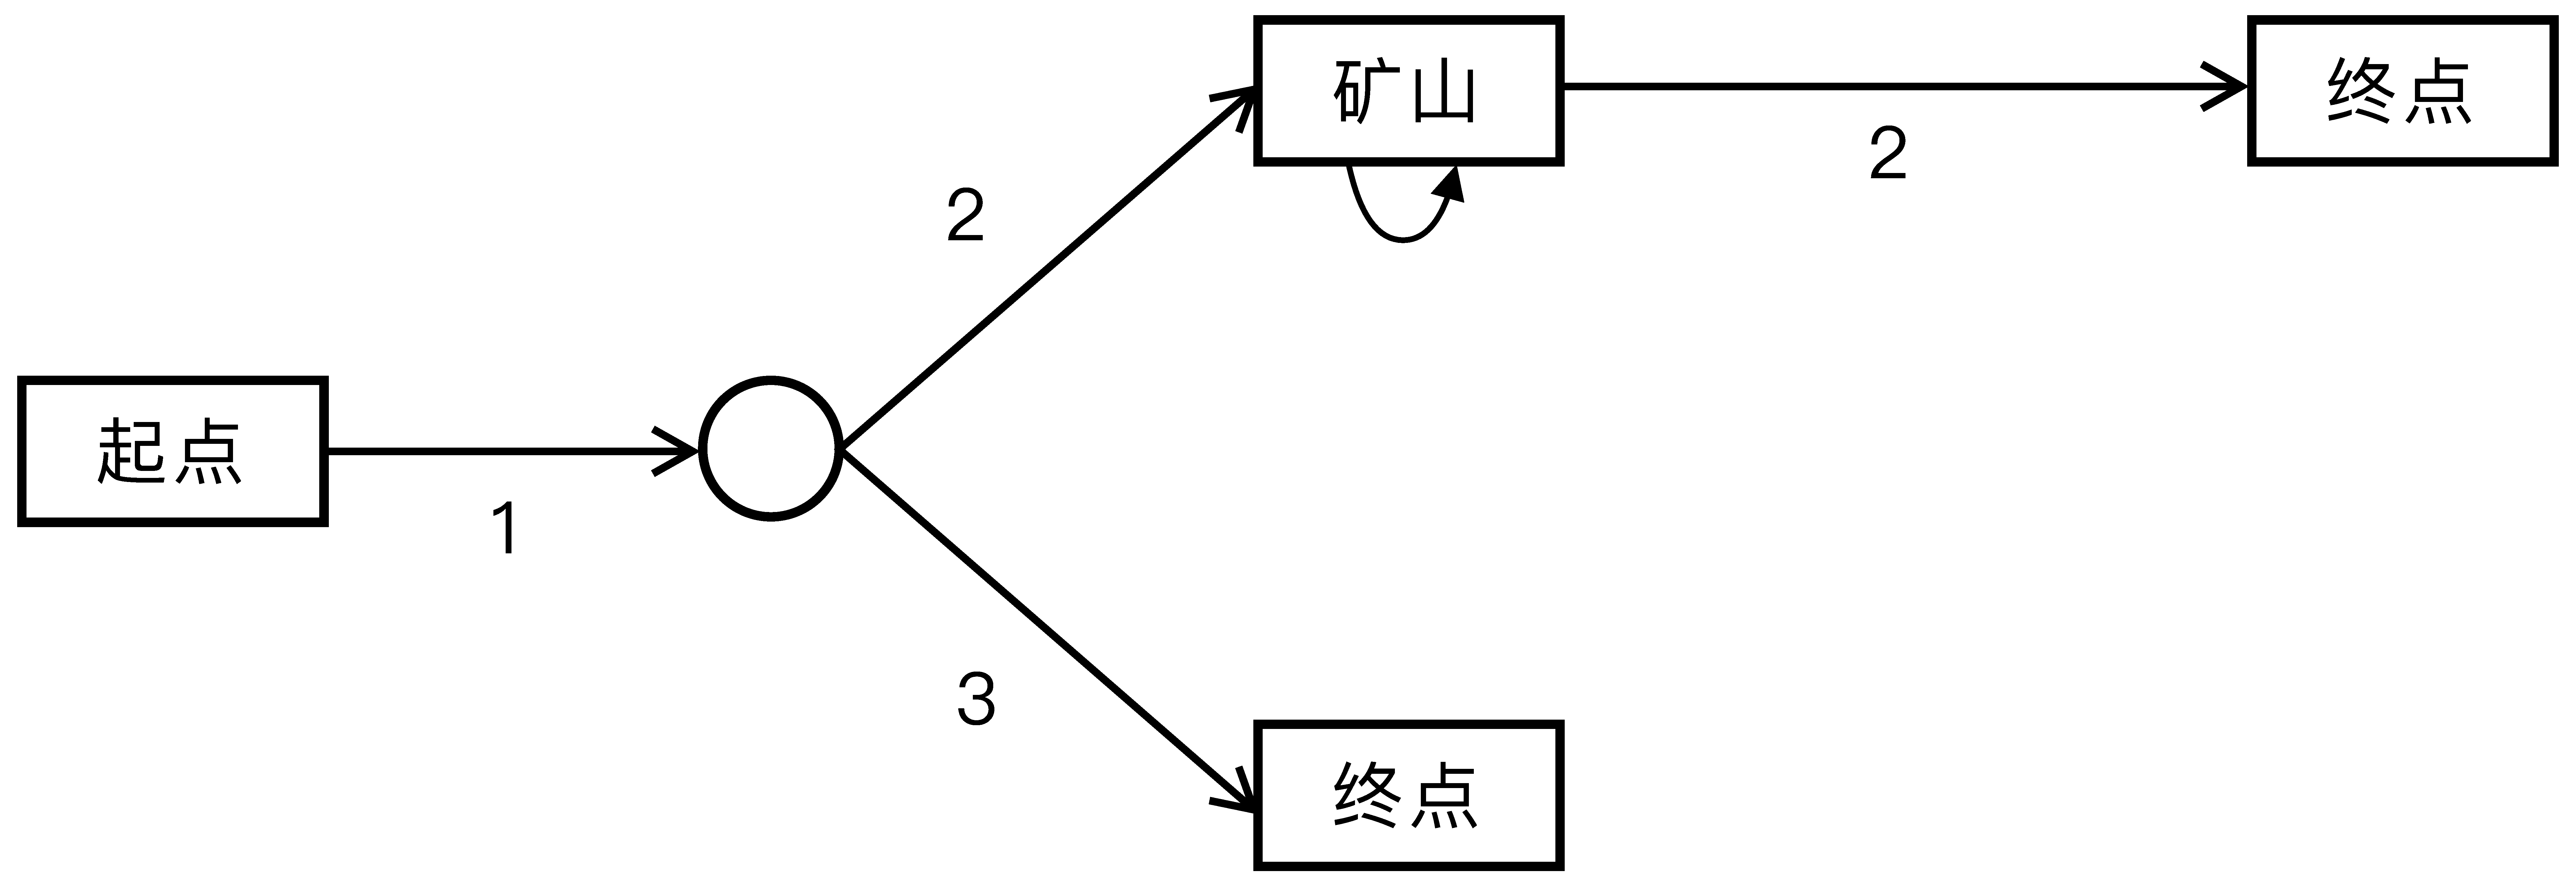
\includegraphics[width=.8\textwidth]{problem3-new-decision}
%     \caption{第三关-考虑中间节点的决策路径}
%     \label{fig:problem3-decision-mid}
% \end{figure}

% 但是根据上面分析可以看到如果收入、花费和绕道的路径满足特定条件,且仅知道当前的天气,未来的天气是未知
% 的,不需要考虑中间路径。
% 因为前往哪里只决定于收益和成本的关系,不决定于某一天当天的的天气,当天的天气只会影响在挖矿阶段玩家
% 的决策。




\subsection{模型求解}

\subsubsection{第三关}

根据\ref{subsec:shortest}的算法可以发现,第三关中玩家到矿山和终点的最短路径中有一个公共位置4,即为关键节点,
简化后的决策路径如图\ref{fig:problem3-decision}所示。
主要考虑的问题是,玩家到达4位置后是否应该前往挖矿、什么样的天气应该挖矿、什么情况应该结束挖矿。

% \begin{figure}[!h]
%     \centering
%     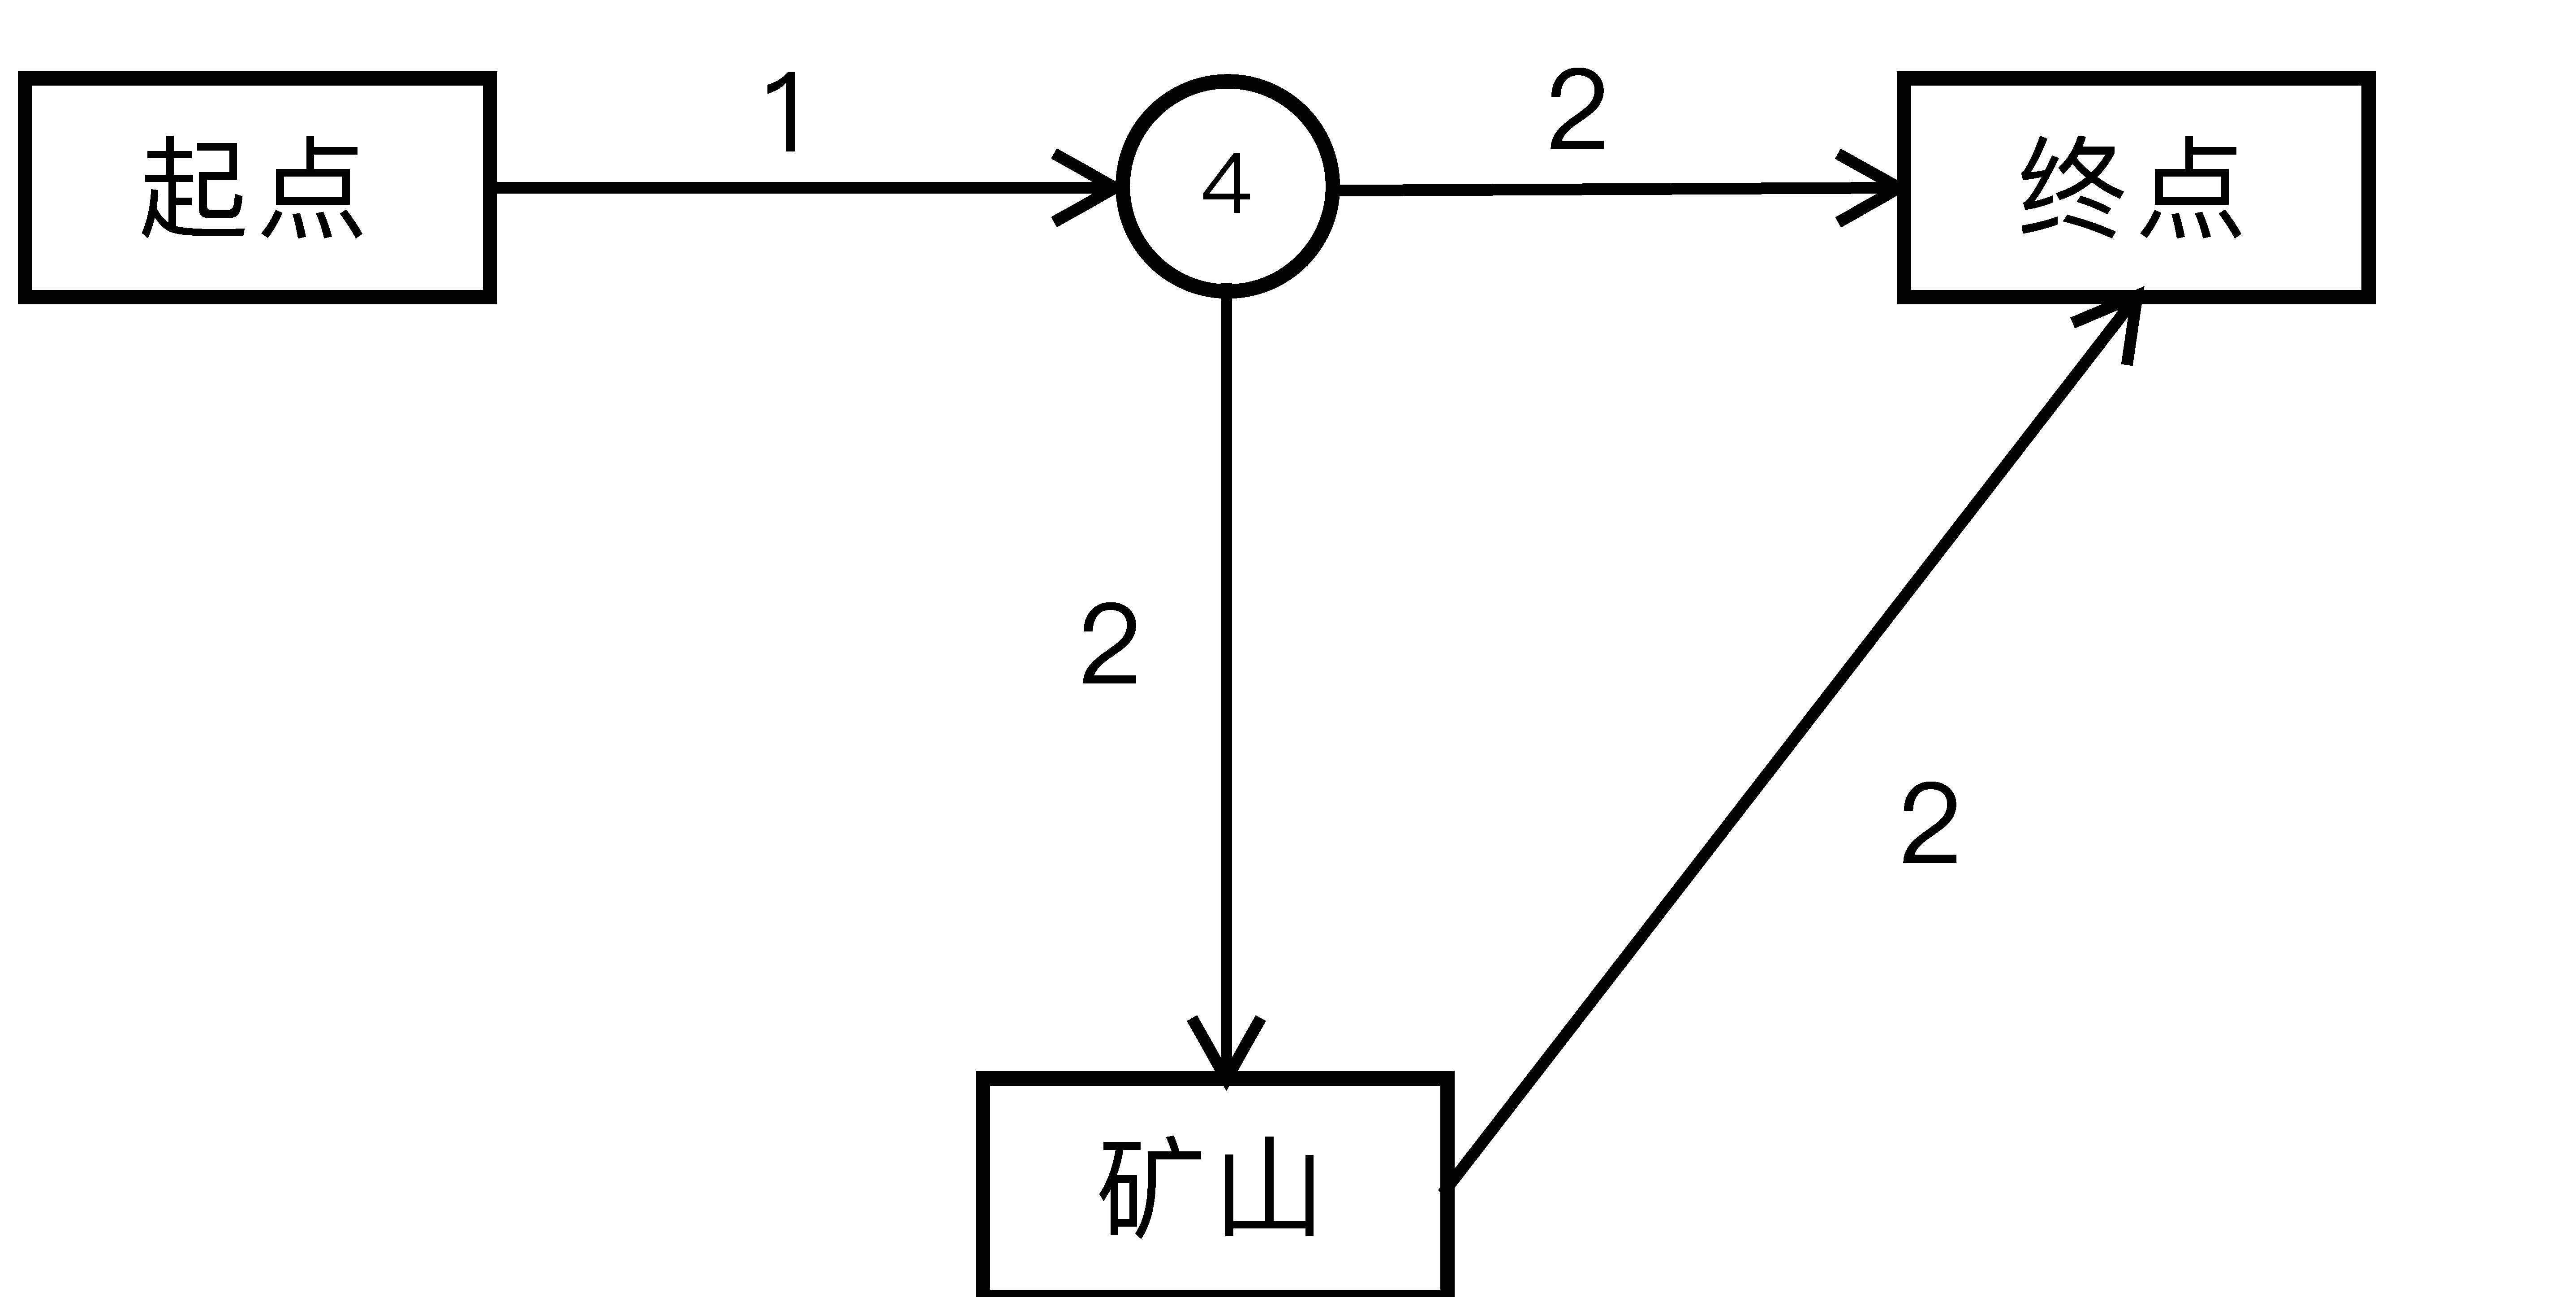
\includegraphics[width=.5\textwidth]{problem3-network}
%     \caption{第三关-模型简化}
%     \label{fig:problem3-network}
% \end{figure}

\begin{figure}[!h]
    \centering
    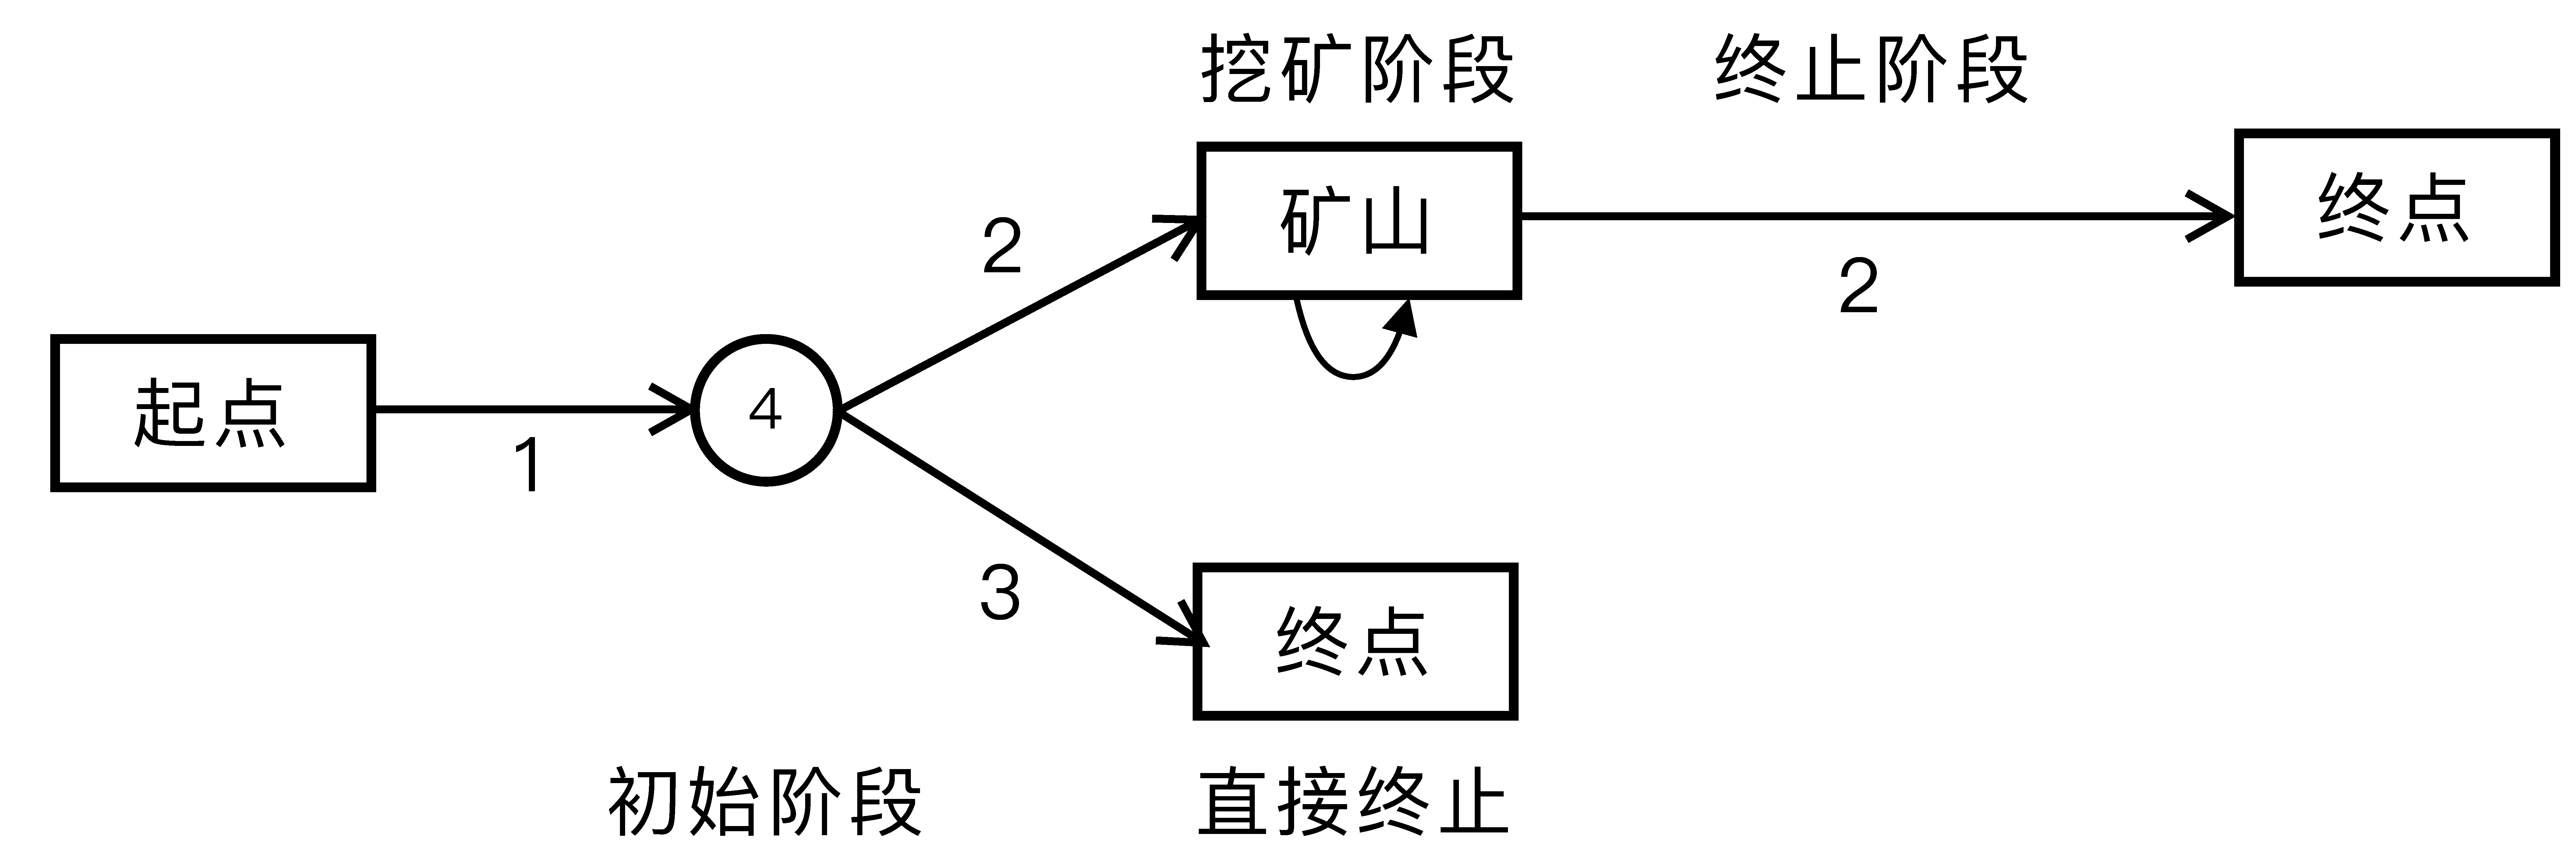
\includegraphics[width=.7\textwidth]{problem3-decision}
    \caption{第三关-决策路径}
    \label{fig:problem3-decision}
\end{figure}

\textbf{(1)成本分析}

该关的基础参数如有,基础收益:$cap_{basic} = 200$元;挖矿绕道距离:$detour = 1$个区块;晴天基础花
费:$c_s=125$元;高温基础花费:$c_{hot}=315$元;总天数$d_{total}=10$天;绕道矿山到终点的最短时
间$d_{min}=5$天。

绕道最高成本$detour*c_{hot}*2=630$元;晴天挖矿收入:$cap_{basic}-3*cost_s=-175$元;热天挖矿
收入:$cap_{basic}-3*cost_h=-745$元;可挖矿天数:$d_{total}-d_{min}=5$天。

\textbf{(2)决策路径分析}

根据上一小节信息,可以比较明显的看到,以挣钱为目的的挖矿是亏损,所以应该准备直接前往终点的资源。
水:$w_{hot}*2*d_{min}=216kg$,粮食:$f_{hot}*2*d_{min}=144kg$。

玩家到达4后需要第一次做决策,如果第1天是晴天,相当于节约了水$(w_{hot}-w_{sun})*2=36kg$,节约了食物
$(f_{hot}-f_{sun})*2=20kg$。

如果到达4后仍然为晴天,则相当于共节约水73kg和食物40kg,由于$detour=1$,所以可以选择绕行到矿山,即前往
3位置,因为即使该天为高温,也能够满足热天走路水54kg和粮食36kg的需求。

玩家到达3后如果再次出现晴天,走到矿山相对于相当于再次节约了水36kg和粮食20kg;到达9矿山后,如果再次出现
晴天,由于上一天节约的水和粮食足够在晴天挖矿的全部消耗,所以应就地挖矿,挣得基础收益200元。

\begin{figure}[!h]
    \centering
    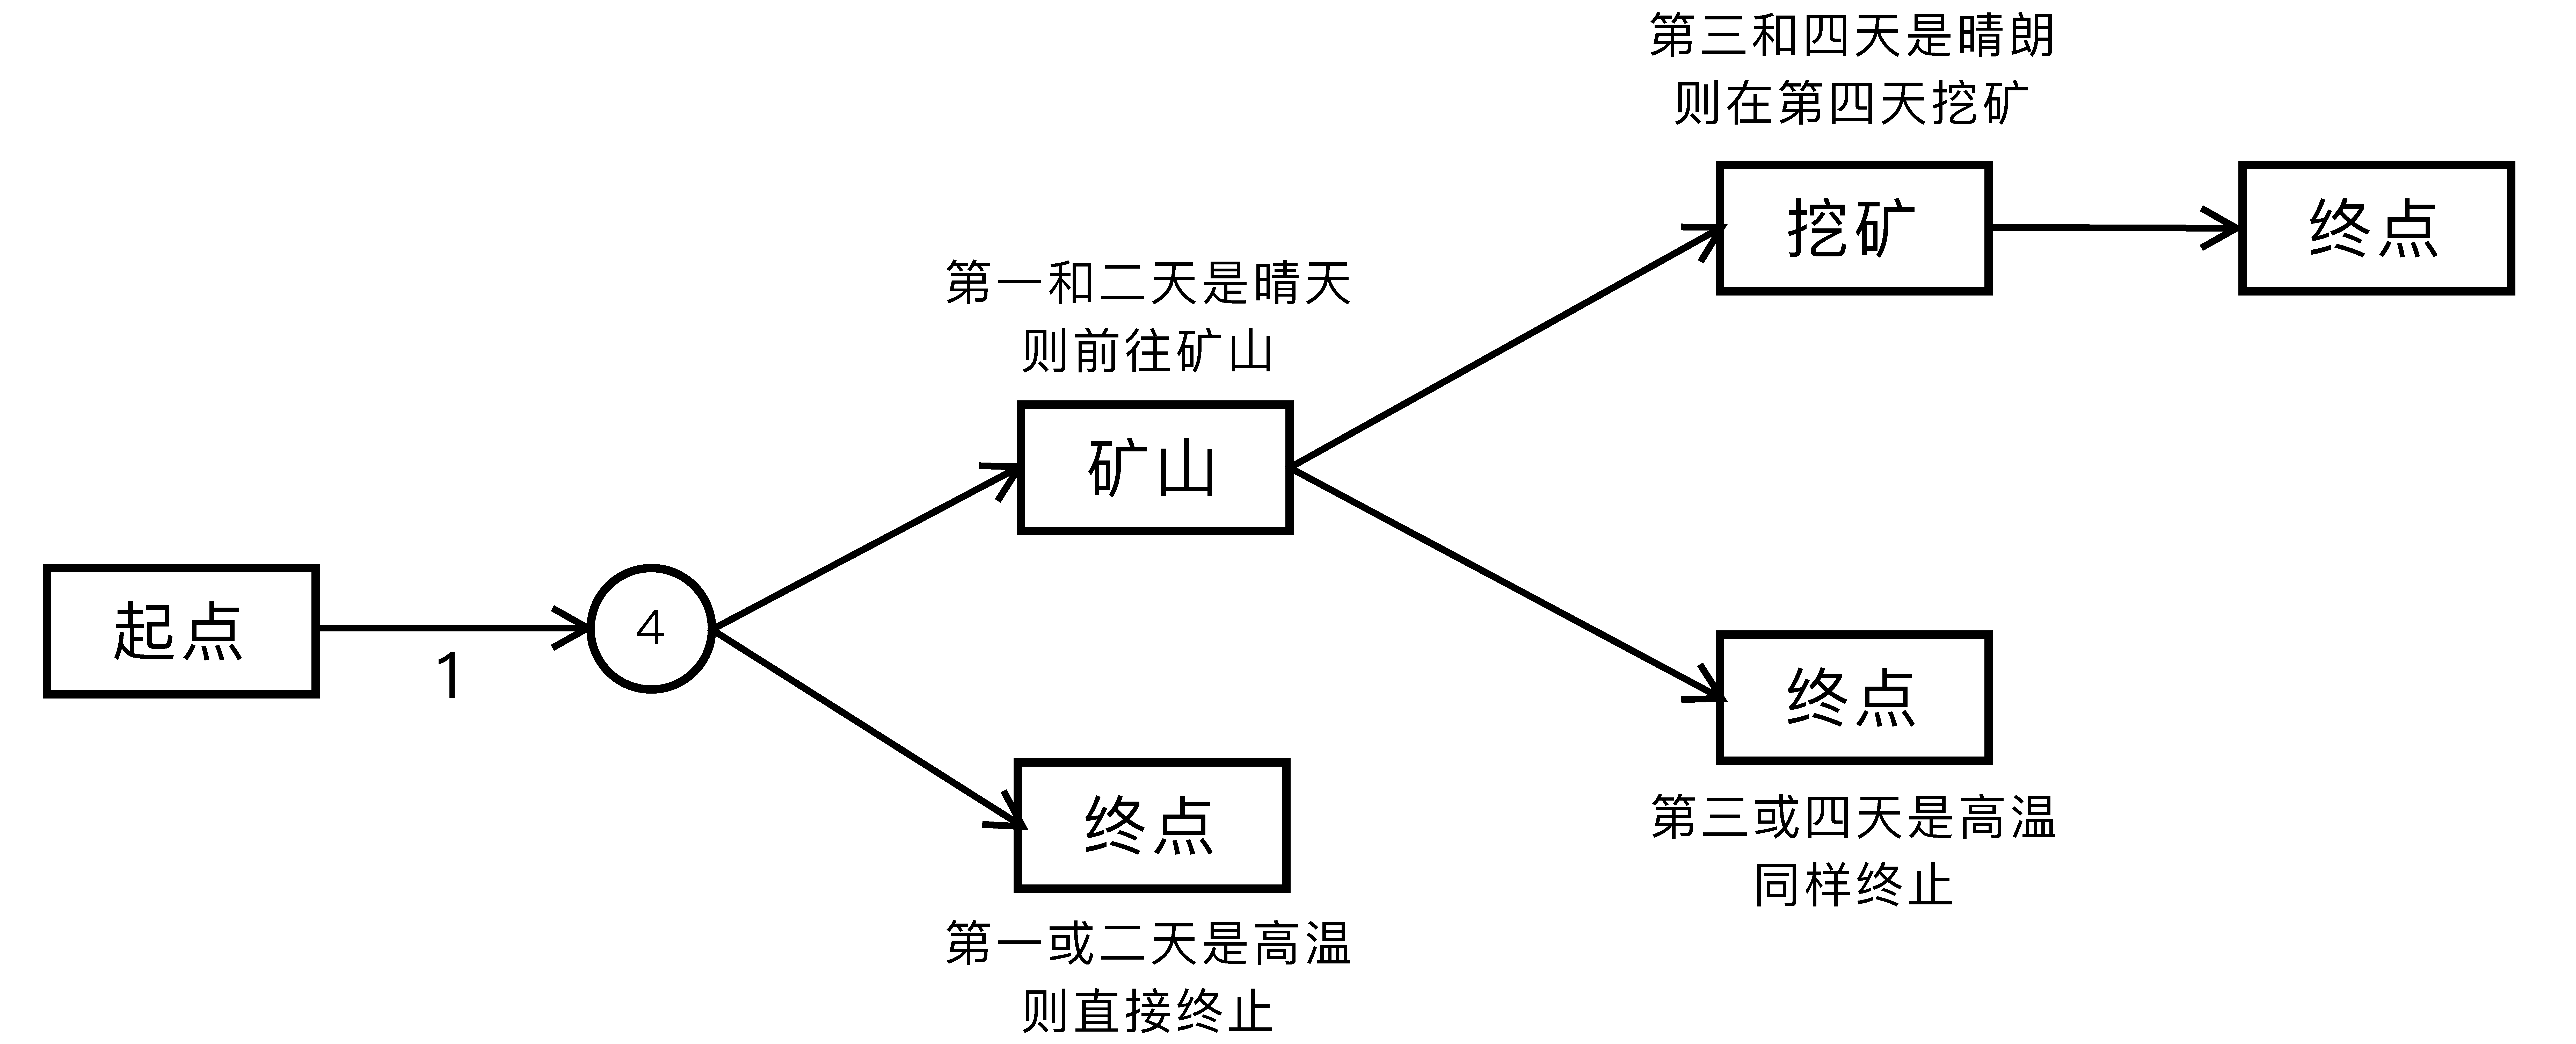
\includegraphics[width=.95\textwidth]{problem3-result}
    \caption{第三关-决策路径选择}
    \label{fig:problem3-result}
\end{figure}

\textbf{(3)策略总结}

上一小节计算出的决策路径呈现的结果即为,准备4天高温行走的粮食和水,如果第1-4天全部为晴天,则在第四天挖矿,获得200元收益。
% 初始的购买总花费为$c_{total} = w_{buy}*w_{cost} + f_{buy}*f_{cost} = 2520$元,购买后剩余资金为
% $m_{left} = m_{init} - c_{total} = 7480$元。

\begin{table}[!htbp]
    \caption{第三关最佳策略}\label{tab:strategy} \centering
    \begin{tabular}{p{2cm}p{13cm}}
        \midrule[1pt]
        初始购买 & $4*w_{hot}=216kg$水和$4*f_{hot}=144kg$的食物,花费2520元 \\
        基本策略 & 第1天前往4号位置,如果第二天是高温,则沿4-6-13到终点;如果第二天不是高温,则按照4-3-9-11-13到终点,其中如果第3/4天全部是晴朗,则在第四天早矿山挖矿 \\
        剩余资金 & 如果没有挖矿,则剩余$m_{init}-216kg*w_{cost}-144kg*f_{cost}=7480$元;如果能够挖矿,则剩余7480+200=7680元 \\
        \bottomrule[1pt]
    \end{tabular}
\end{table}





\subsubsection{第四关}

根据上文分析,第四关决策路径如下图,需要对在矿山的挖矿成本进行量化后,判断其在几个核心的决策节点,
应该作出什么决策,同时计算何时应该前往终点。

\begin{figure}[!h]
    \centering
    
\includegraphics[width=.9\textwidth]{problem4-decision}
    \caption{第四关-决策过程}
    \label{fig:problem4-decision}
\end{figure}

\textbf{(1)成本分析}

该关的基础参数如有,基础收益:$cap_{basic} = 1000$元;挖矿绕道距离:$detour = 0$个区块;
晴朗天气基础消费$c_{sun}=125$元,炎热天气基础消费$c_{hot}=315$元,沙尘暴天气基础消费$c_{hot}=350$元

收入方面,由于在村庄购买的物品价格翻倍,挖矿获得的收入应该分为起点购买的资源用完前,和资源用完后。
在资源用完前,与第三关结果一致,晴天挖矿挣635元,高温挖矿挣55元,同时沙尘暴挖矿损失50元;
资源用完后,晴天收益为$cap_{basic}-c_{sun}*2*3=370$元,高温挖矿收益$cap_{basic}-c_{hot}*2*3=-890$元,
沙尘暴挖矿收益为$cap_{basic}-c_{dust}*2*3=-1100$元。

\textbf{(2)决策路径基础分析}

% 该问题的路径决策主要有,是否应该挖矿、应该先去村庄还是矿山、什么天气可以在矿山挖矿、是否应该去及多久应该去
% 村庄、在村庄应该购买多少资源、多久应该前往终点。

使用起点购买的资源挖矿时,天晴和高温的净收益分别为635元和55元,虽然沙尘暴天气损失50元,但是题目条件是该天气比较
少,所以在矿山挖矿我们可以视为能够获取收益。
按照天气最恶劣的情况计算,1200kg的负重也足够起点到终点,并剩余可以用来挖矿的资源。
同时$detour=0$,即起点到终点的最短路径是可以直接经过矿山,所以玩家应该在起点购买足够的资源,在路过矿山时直接挖
矿以获取收益。

但是在资源耗尽后,高温天气亏损近晴天收益的两倍,同时从矿山前往村庄的过程需要消耗大量资源,玩家也只知道当天的天气,
不知道未来是否是高温,所以完全使用村庄的资源挖矿是不合算的。
不过需要考虑的是,由于晴朗天气与高温天气的食食物和水的消耗比例不一致,可能会使得前往村庄购买资源是划算的。

% 从起点到矿山一共经过5个区块,最恶劣的天气可以视做消耗5天炎热与1天沙尘暴,共计消耗500kg的资源;
% 从矿山前往终点我们同样预设1次沙尘暴,外加3天高温,共计消耗320kg的资源,初始携带1200kg的食物和水,假设按照1:1
% 携带,也能够剩余足够的资源挖矿。

\uline{综上,玩家一般情况下应该选择最短的路径直接前往矿山挖矿,且不应该存粹使用村庄资源挖矿,使用资源不均的问题下一节讨论。}

\textbf{(3)购买策略与决策路径}

在起点处资源的购买应该满足1200kg,考虑到沙尘暴和高温消耗箱数水:食物=1:1,按照该比例购买,恰好水购买720kg,食物
购买480kg,也可以按照晴朗天气的消耗比例购买,后续进行分析。

如果全部是高温,最终资源会被按比例恰好消耗;但是如果在13号位置前或19号位置上,先前碰到的全部是晴朗天气,水和食物的比例将失衡,
可能会产生其他决策方式。
但是不管是否有足够的水多余,玩家都不应该前往村庄购买食物。
当玩家的食物全部在村庄购买时,水无需购买的情况下,其挖矿的基础成本为$f_{cost}*2*f_{hot}*3=1080$元,即就算不需要买食物,使
用村庄购买的食物挖矿在高温天气挖矿亏损的。

在食物无需购买,水需要在村庄购买时,高温挖矿基础成本为$w_{cost}*2*w_{hot}*3=810$元,去村庄购买水去挖矿能够获取收益,但是玩家
购买需要绕行以及额外的费用,比如从19号前往14号位置为例,在14号购买水并出行后需要前往矿山挖矿弥补该消费,如果连续遇到高温和沙暴天
气,经过简单的计算即可知,玩家无法获得额外收益。

\uline{综上所述,不管天气如何变化,都不应该前往村庄购买水和食物}。最终的具体的决策路径与最佳策略为:

% 这时可能可以先前往村庄,再
% 前往矿山,此时的$detour=2$;或在资源用完后选择前往村庄购买食物,再返回矿山,此时的$detour=4$。
% 如果到达13号位置时,前4天全部是晴朗,会导致水多出8箱,即使第五天仍然为晴朗,也不应该前往村庄,因为多余的水不足以支
% 付$detour=2$所花费的可能费用。

\begin{table}[!htbp]
    \caption{第四关最佳策略}\label{tab:strategy} \centering
    \begin{tabular}{p{2cm}p{13cm}}
        \midrule[1pt]
        初始购买 & 720kg水和480kg的食物,或按照晴朗天气消耗比例 \\
        基本策略 & 直接前往矿山,除了沙尘暴其他天气保持前进,到达矿山后不管天气如何都选择挖矿 \\
        结束条件 & 如果挖矿过程中剩余的水将小于192kg或粮食小于128kg,选择沿最短路径前往终点 \\
        \bottomrule[1pt]
    \end{tabular}
\end{table}

\begin{figure}[!h]
    \centering
    
\includegraphics[width=.7\textwidth]{problem4-result}
    \caption{第四关-决策路径选择}
    \label{fig:problem4-decision}
\end{figure}



\section{多玩家博弈条件下的策略}
\label{sec:simulate}


\subsection{问题分析}

本问题中,游戏中存在多个决策者,每个决策者维护各自的的决策变量与目标函数,且决策者的行为相互影响,故我们使用博弈模型进行研究。

在第五关,玩家个数为2,每位玩家在第0天都拥有完全信息,且每位玩家的行动方案需在第0天确定且此后不能更改,形成\textbf{完全信息静态博弈}的局面。在静态模型的分析框架下,我们需要确定博弈的局中人、决策集合、效用函数、赢得矩阵,从而计算出博弈的纳什均衡,制定最优的游戏策略。

第六关,玩家个数为3,每名玩家在当天行动结束后均知道其余玩家当天的行动方案和所剩资源数量,随后确定各自第二天的行动方案。与第五关相似的是,每位玩家都希望从起点走一条到终点的最优路径。但与第五关不同,第六关玩家每一步都要做决策,即根据每一天的环境重新规划一条对自身最有利的路线,即可以抽象为玩家与环境互动与反应,可以用\textbf{马尔可夫决策过程}理论工具进行分析。


\subsection{第五关模型建立及求解}

\subsubsection{模型建立}
我们首先针对第五关建立完全信息静态博弈模型。

\textbf{(1)局中人}

在一局对策中,有权决定自己行动方案的对策参加者,称为局中人。在本模型中局中人即玩家。我们用 $I$ 表示局中人的集合。

\textbf{(2)决策集合}

一局对策中,可供局中人选择的一个实际可行的完整的行动方案称为一个策略。参加对策的每一局中人$ i\ ,\ \ i\ \epsilon\ I\ $ ,都有自己的决策集合$ D_i $。

\textbf{(3)赢得矩阵}

双方每一种满足$ x_1 \in D_1, x_2 \in D_2$的决策$({\ x}_1,\ x_2\ )$,用$u({\ x}_1,\ x_2\ )$来表示局中人在本轮博弈产生的效用。使用赢得矩阵$ M={\ |\ u(i,\ j)\ |\ } $来表示所有博弈可能性的收益。

\textbf{(4)纳什均衡}

博弈双方都力求通过决策让自己在游戏中的效用最大化,用$ {x_1}^\ast,\ {x_2}^\ast $ 分别表示玩家1和玩家2会选择的的策略。
寻找满足
\begin{equation}
    \begin{cases}
 u_1({x_1}^\ast\ ,\ {x_2}^\ast)\ \geq\ u_1(x_1\ ,\ {x_2}^\ast)  \\
 u_2({x_1}^\ast\ ,\ {x_2}^\ast)\ \geq\ u_2({x_1}^\ast\ ,\ x_2\ )  \\
 x_1\ \epsilon\ D_1\  \\
 x_2\ \epsilon\ D_2\  \\
    \end{cases}
\end{equation}
的策略组合即为本问题的纳什均衡$ x^\ast\ =({x_1}^\ast\ ,\ {x_2}^\ast)\ $。

\subsubsection{模型求解}\label{p5_solution}

\begin{figure}[!h]
    \centering
    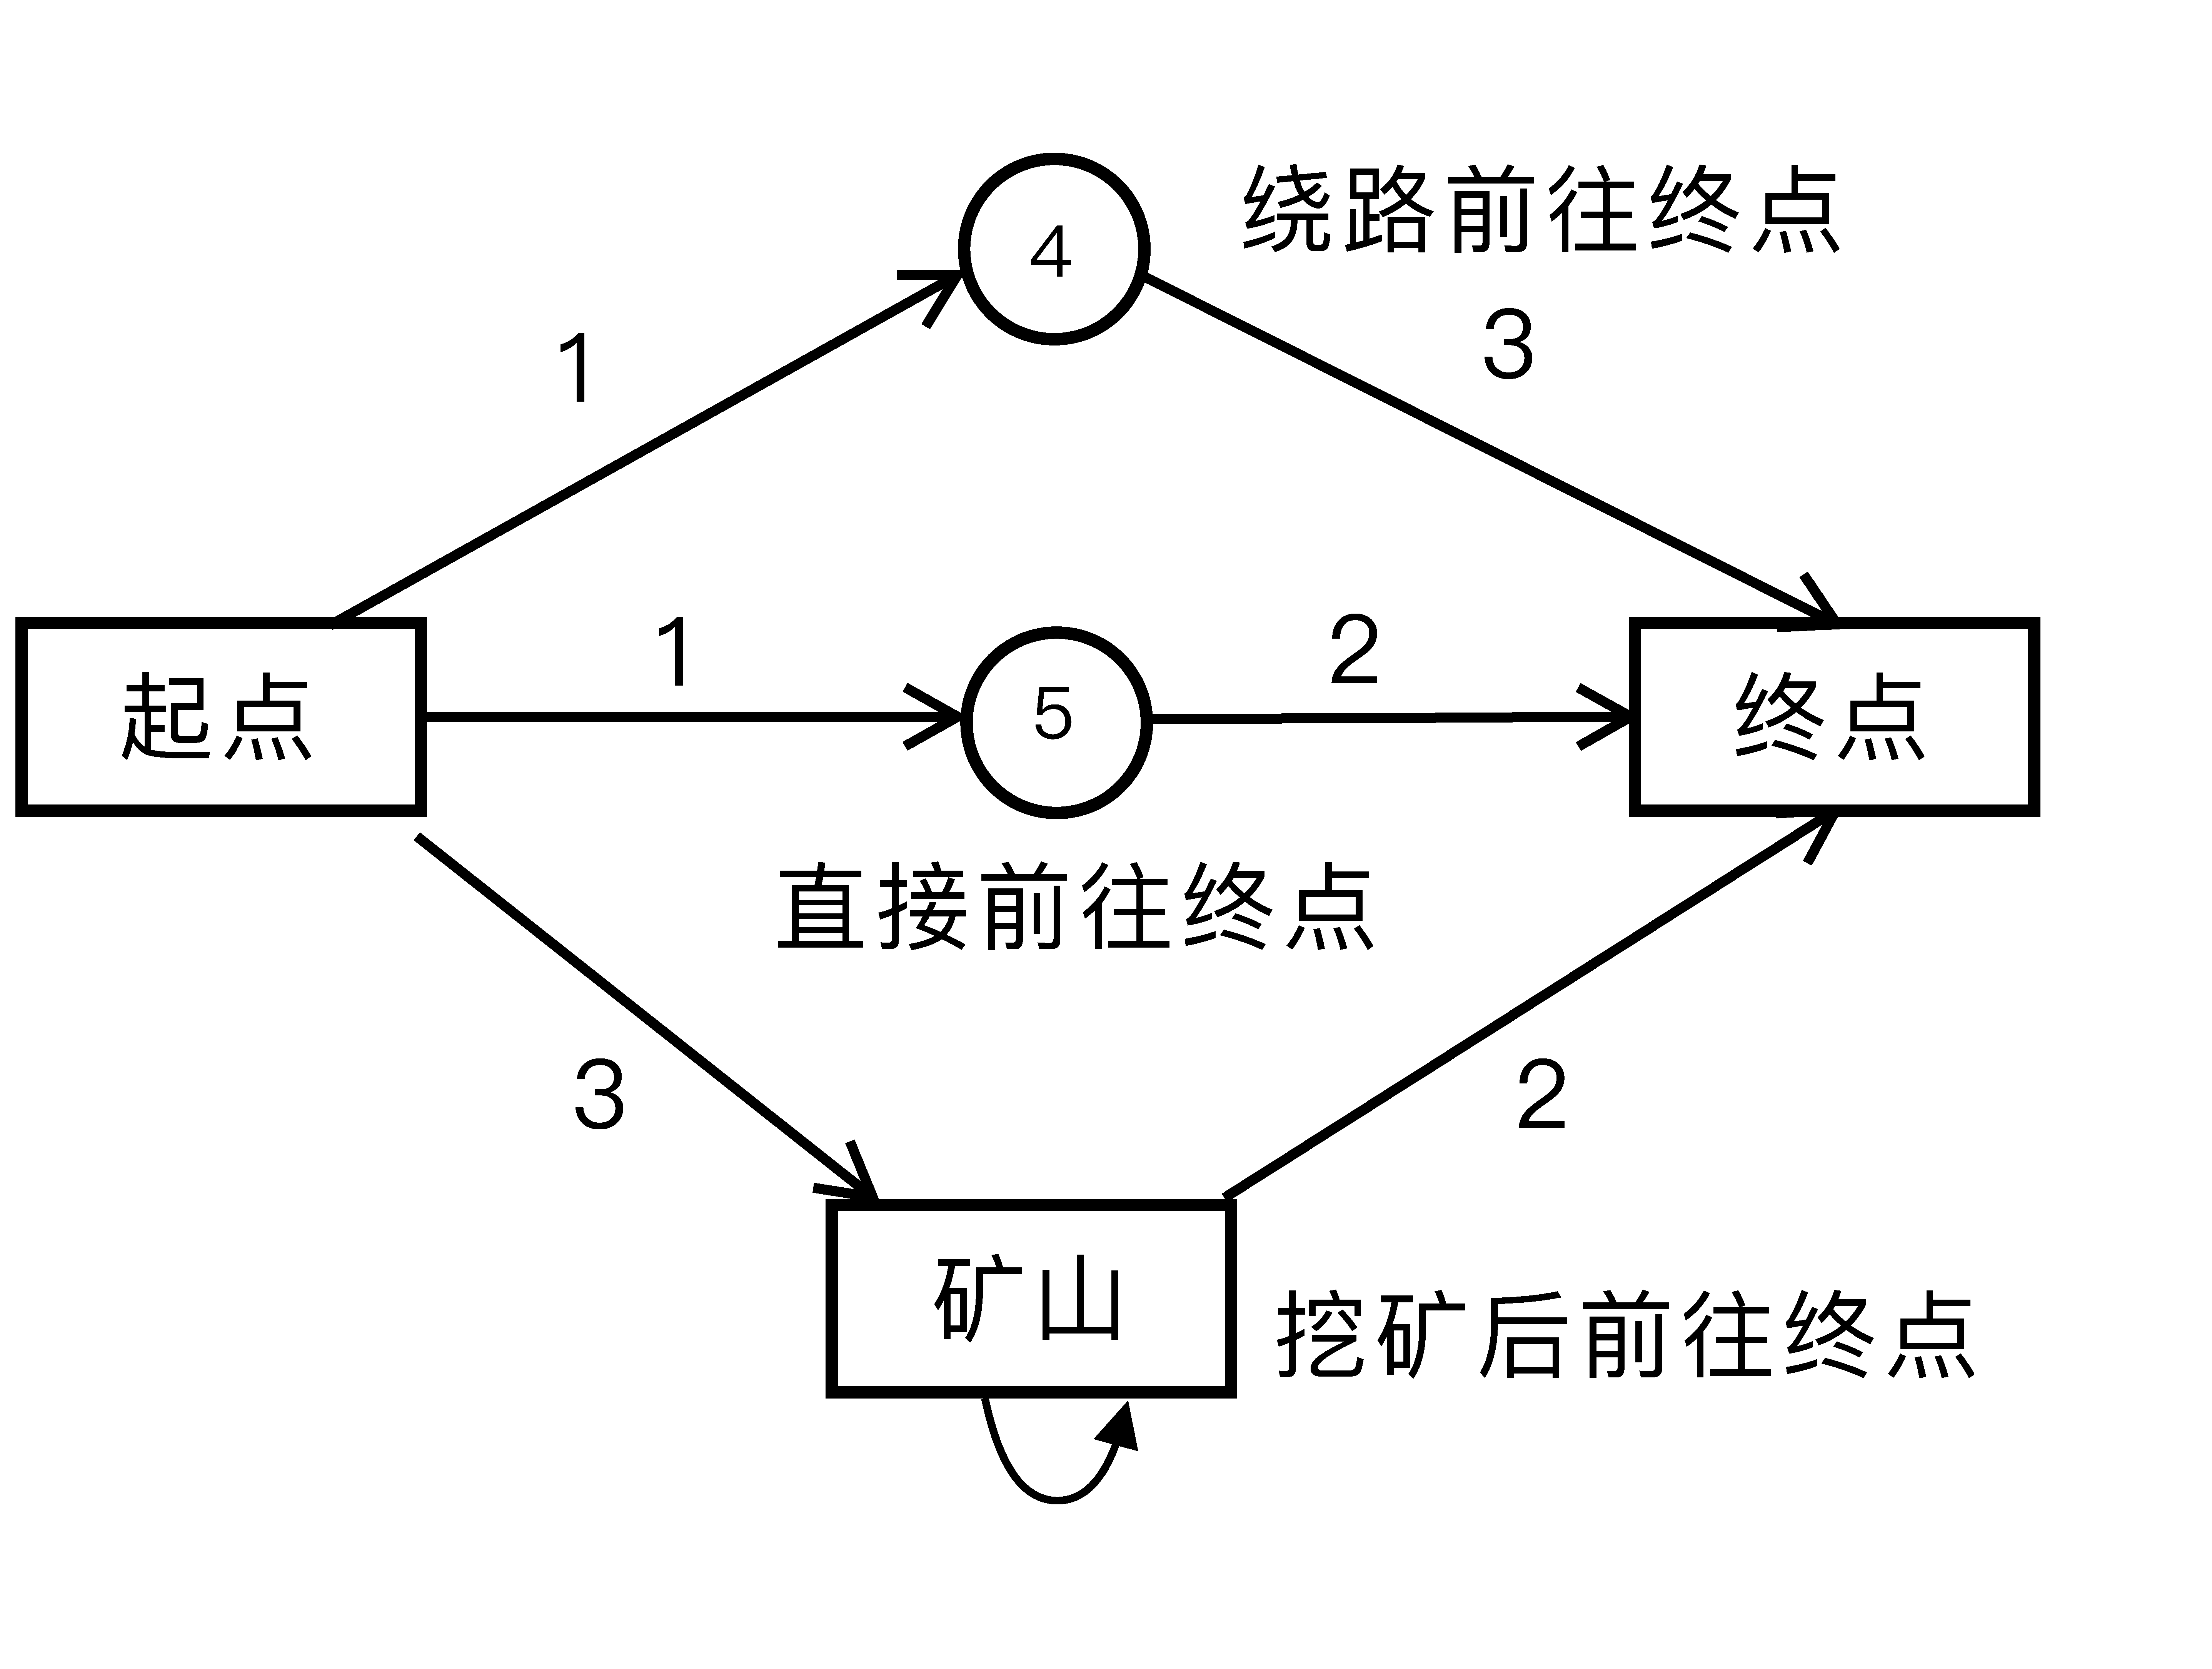
\includegraphics[width=.550\textwidth]{problem5-network}
    \caption{第五关:决策路径选择}
    \label{fig:problem5-network}
\end{figure}

为了得出本问局中人的策略集,我们先考虑只有一位玩家的情况。在本文预设的游戏中,局中人的目标都是在规定时间内到达终点,并挣取尽可
能多的资金。一般的最优策略为前往矿山挖矿,局中人在前往矿山的路径与挖矿日期的选择上进行博弈。但第五关的前提条件特殊,由于挖矿
收益较低,且天气情况已经给定,经过前文所建立的动态规划模型并求解,发现采取挖矿策略最终剩余金额为9325元。相比之下,从起点直接
前往终点最终剩余金额为9535元。在如此的前提条件下,对于局中人而言最优的策略不再是挖矿,而是直接以最近的路径返回终点。

\begin{table}[!htbp]
    \caption{一名玩家的策略}\label{tab:p5strategy1} 
    \centering
    \begin{tabular}{ccc}
        \toprule[1.5pt]
        策略编号 & 策略描述 & 最终金额 \\
        \midrule[1pt]
        策略1 & 先挖矿后前往终点 & 9325元 \\
        策略2 & 不挖矿直接前往终点 & 9535元\\
        策略3 & 不挖矿绕路前往终点 & 9425元\\
        \bottomrule[1.5pt]
    \end{tabular}
\end{table}

随后我们引入博弈的情况。经计算,本问中玩家无论是直接前往终点还是挖矿,最优解背包容量都不会超过最大限制,所以玩家的目标仅仅关
注如何让结束时的剩余金额最大化,即都希望采取直接从起点尽快前往终点的策略。但当游戏中2个玩家都采取这一策略,那么由于游戏规则
的限制,他们各自的结果经计算得为9070元,劣于单独直接前往终点的结果9535元,且劣于单独前往挖矿的结果9325元。

\begin{table}[!htbp]
    \caption{两名玩家策略相同的情况}\label{tab:p5strategy1} 
    \centering
    \begin{tabular}{ccc}
        \toprule[1.5pt]
        策略编号 & 策略描述 & 两玩家各自最终金额 \\
        \midrule[1pt]
        策略4 & 两玩家都先挖矿后前往终点 & 8515元 \\
        策略5 & 两玩家都不挖矿直接前往终点 & 9070元\\
        策略6 & 两玩家都不挖矿绕路前往终点 & 8850元\\
        \bottomrule[1.5pt]
    \end{tabular}
\end{table}

最终我们将游戏决策描述为以下的博弈问题:
\begin{enumerate}
    \item 博弈的参与者(局中人)为2名玩家;
    \item 博弈的策略有3种:直接前往终点、绕路前往终点、挖矿后前往终点;
    \item 博弈的2名局中人面临的决策集相同;
    \item 博弈双方的目的都是成功抵达终点并使得剩余金额最大;
\end{enumerate}

博弈决策的行动及其产生的结果如下表显示:

\begin{table}[!htbp]
    \caption{两名玩家博弈下的最终金额}
    \centering
    \begin{tabular}{cccc}
        \toprule[1.5pt]
         玩家2 / 玩家1 & 直接前往终点 & 绕路前往终点 & 挖矿后前往终点  \\ 
        \midrule[1pt]
         直接前往终点 & 9070, 9070 & 9425, 9535 & 9325, 9535 \\ 
         绕路前往终点 & 9535, 9425 & 8850, 8850 & 9325, 9425 \\
         挖矿后前往终点 & 9535, 9325 & 9425, 9325 & 8515, 8515  \\  
        \bottomrule[1.5pt]
    \end{tabular}
\end{table}

我们将玩家1可能的决策记作$ x_1\ \epsilon\ D_1\ =\ {1,\ 2,\ 3\ } $,分别表示直接前往终点,绕路前往终点与
挖矿后前往终点。同样玩家2可能的决策记作 $x_2\ \epsilon\ D_2\ =\ {1,\ 2,\ 3\ }$。

玩家1的效用函数可以用赢得矩阵
\begin{center}
    $ M_1={\ |\ u_1(i,\ j)\ |\ }_{3\times3\ }=\ \left(\ \begin{matrix}9070&9425&9325\\9535&8850&9325\\9535&9425&8515\\\end{matrix}\ \right) $
\end{center} 
表示。同样,玩家2的赢得矩阵为
\begin{center}
    $ M_2={\ |\ u_2(i,\ j)\ |\ }_{3\times3\ }=\ \left(\ \begin{matrix}9070&9535&9535\\9425&8850&9425\\9325&9325&8515\\\end{matrix}\ \right) $
\end{center}

容易解得本题的纳什均衡的策略为$\ (2\ ,\ 1)$ 或 $(1\ ,\ 2)$,即玩家1选择绕路前往终点、玩家2选择直接前往终点,或玩家1选择直接前往终点、玩家2选择绕路前往终点。如果玩家间的决策有先后且相互信息完全公开,那么后决策的玩家在得知先决策的玩家的决策结果后一定会按照纳什均衡进行决策。

然而,本题中玩家需同时做出决策且不能沟通。由于上述博弈存在2个纳什均衡,因此无法求出最优决策。进一步考虑,用概率刻画玩家的行为,可求出混合策略。由于在本文中玩家1与玩家2面对的条件相同,故我们仅分析玩家1的决策。设玩家1采取行动$ \ i\ $的概率为 $ p_i(i\ =\ 1\ ,\ 2\ ,\ 3\ )\ $,设玩家2
采取行动$ \ i\ $的概率为 $ q_i(i\ =\ 1\ ,\ 2\ ,\ 3\ )\ $,则玩家1
的混合策略集为
\begin{equation}
    D_1\ =\ {\ p\ =\ (p_1,\ {\ p}_2,\ {\ p}_3)\ \ |\ \ 0\le p_{i\ }\le1\ ,\ \sum_{i=1}^{3}p_i\ =\ 1\ } 
\end{equation}

定义混合策略下玩家1的效用期望为
\begin{equation}
    U_1(p,\ q)=\ pM_1q^T\ =\ \sum_{i=1}^{3}\sum_{j=1}^{3}{p_im_{ij}q_j}
\end{equation}

期望效用最大化,其面临的决策问题是
\begin{equation}
     \max \quad  {U_1(p\ ,\ q)},  \quad {p\in S_1}
\end{equation}

使用Lingo解得
\begin{center}
    $p_1=0.609$,  \quad 
    $p_2=0.301$,  \quad 
    $p_3=0.090$
\end{center}

在重复多次游戏的情况下,若玩家以60.9\%的概率选择策略1,以30.1\%的概率选择策略2,以9\%的概率选择策略3,此时玩家的期望效用是最高的。若只面对一局游戏,则玩家只能做出一次决策。把最有可能得到令效用最大化的选择作为最佳策略,得到第五关的最佳策略为:
\begin{table}[!htbp]
    \caption{第五关最佳策略}\label{tab:strategy} \centering
    \begin{tabular}{p{2cm}p{13cm}}
        \midrule[1pt]
        初始购买 & 81kg水和66kg的食物 \\
        决策路径 & 沿着到终点的最短路径,第1日移动,第2日停留,第3日移动,第4日移动,第5日到达终点 \\
        \bottomrule[1pt]
    \end{tabular}
\end{table}

\subsection{第六关模型建立及求解}

\subsubsection{模型建立}
首先我们对玩家的行为作出如下假设:

\begin{enumerate}
    \item 玩家都是理性玩家,目标都是以最大化的剩余金额赢得游戏;
    \item 玩家在决策前没有交流,无法产生勾结、合作;
    \item 所有玩家同时决策;
    \item 不考虑玩家之间的恶意竞争,即故意与其他玩家同走一条路径以达到消耗对方资源的目的。
\end{enumerate}

采用马尔可夫决策过程进行分析。马尔可夫决策过程是一个智能体采取行动从而改变自己的状态获得奖励并与环境发生交互的循环过程。在本问中将玩家看作智能体,对整个游戏的环境与条件有着完全的感知能力,其下一步的操作完全根据当前状态决策,体现了马尔可夫性。

我们将马尔可夫决策过程如下表示:$ M = < S, X, P_{s,x}, R > $

\textbf{(1)状态集合}

我们用$ \ s_k\ \in S_k $ 表示第$k$阶段有限状态的集合,即当前局势的所包含的一切可供决策的信息。与\ref{dp}小节动态规划模型中所指的状态不同,此处的状态不仅包括玩家自身的信息,还包括了其他玩家的行动方案和剩余资源数量。与以玩家1为例,状态集合如表\ref{tab:MDPS_states}所示:
\begin{table}[!htbp]
    \caption{状态集合包含的状态信息}\label{tab:MDPS_states} \centering
    \begin{tabular}{cc|cc}
        \toprule[1.5pt]
        编号  & 状态信息 & 编号 & 状态信息\\
        \midrule[1pt]
        $A$ & 本人金钱     & $G$ & 玩家3金钱 \\
        $B$ & 本人剩余资源  & $H$ & 玩家3剩余资源\\
        $C$ & 本人背包容量  & $I$ & 玩家3当日策略 \\
        $D$ & 玩家2金钱    & $J$ & 天气 \\
        $E$ & 玩家2剩余资源 & $K$ & 游戏基本参数 \\
        $F$ & 玩家2当日策略 & $L$ & 游戏基本地图 \\
        \bottomrule[1.5pt]
    \end{tabular}
\end{table}

\textbf{(2)动作集合}

我们用$ \ x_k\ \in X_k $第$k$阶段表示动作的集合。本问的地图为矩形方格,当玩家处于地图的任意一个格子中,其都处于一个初始
状态$S_{0,j} ,j\in \{ 1,2 \}$,其可以向地图上下左右任意做出动作进入下一个状态$ S'_{i,j},i\in \{1,2,3,4\} ,j\in \{ 1,2 \} $。
如果不考虑其他玩家,那么当前玩家就会按照最优策略决策下一步动作。但若引入多个玩家,当两个或多个玩家的最优决策指向地图上同一个格子,
如图\ref{fig:problem6-game}所示,那么这一轮动作将会带来博弈。

\begin{figure}[!h]
    \centering
    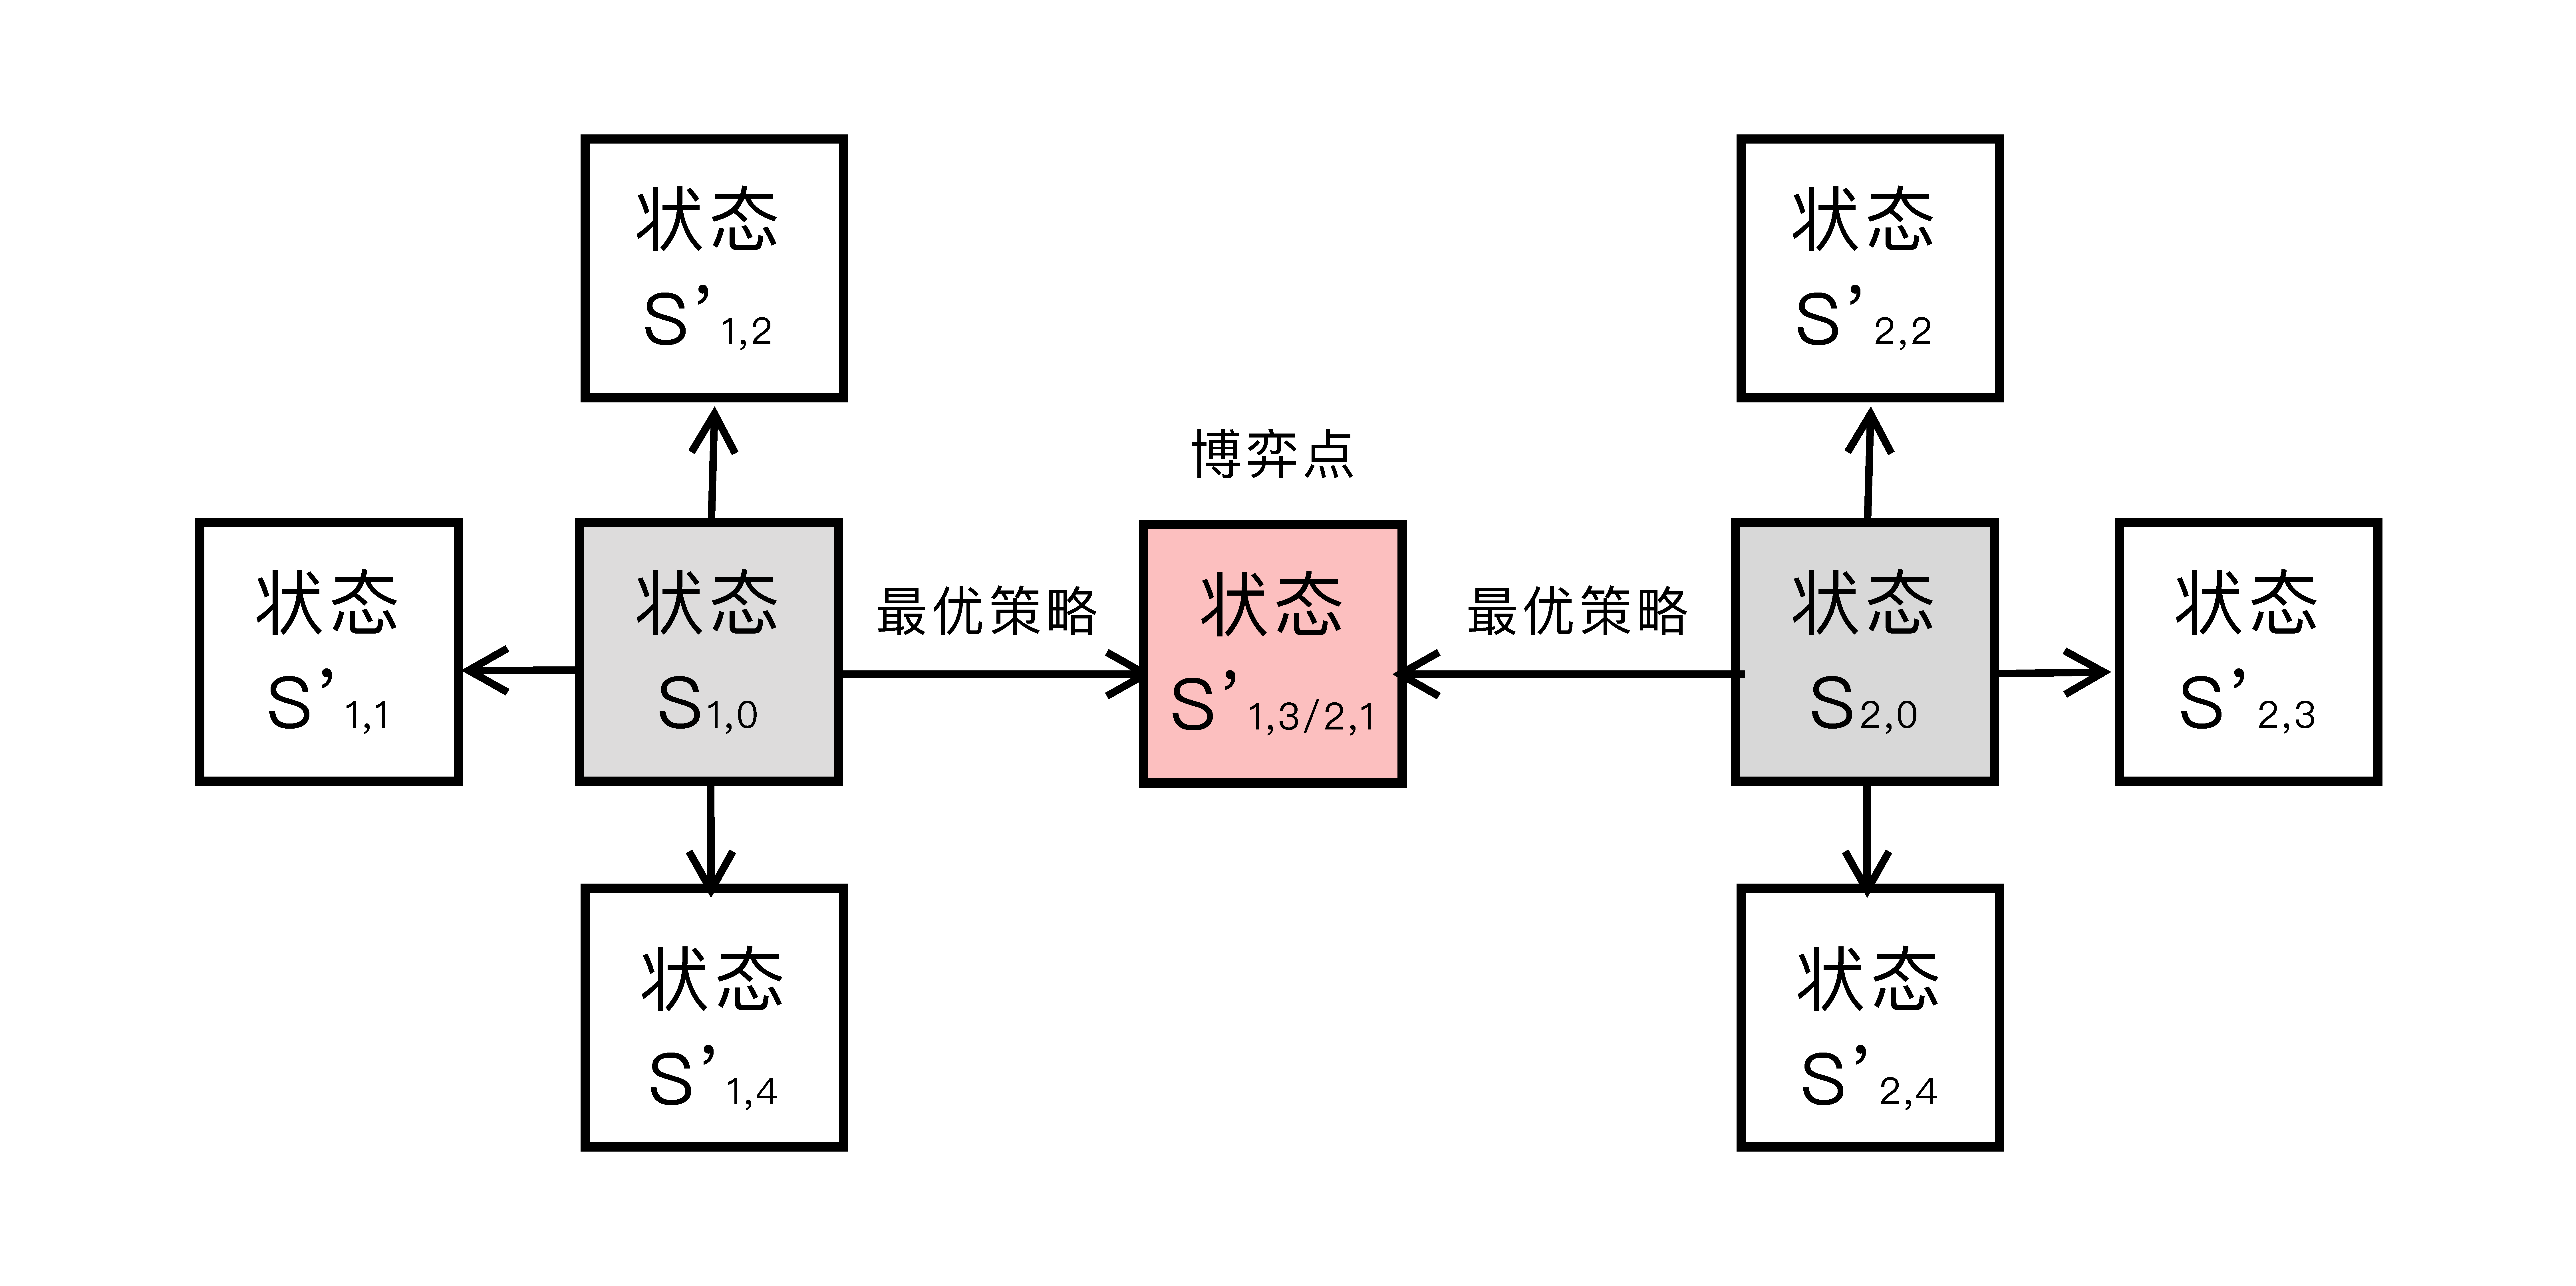
\includegraphics[width=.8\textwidth]{problem6-game}
    \caption{第6关:动作集合与博弈示意图}
    \label{fig:problem6-game}
\end{figure}

在继续讨论之前,首先要分析玩家在面临博弈冲突时会做出怎样的选择。从对第五关的讨论中可以看出,混合策略求解的是收益均值最大化下的决策概率,但任意某一局的策略仍旧是不确定的。因为从多盘游戏的趋势来看,所有玩家的初始条件相同,若都选择以最优的策略进行决策,经过足够多次的博弈,他们的所有局数资金之和应当是逐渐趋同的。通过仿真实验可对这一推论进行验证,构建第五关的游戏环境,令玩家1与玩家2以\ref{p5_solution}小节中求出的概率制定策略,重复进行5000次游戏,玩家1的资金数占两人总资金数的比例随游戏次数的变化关系如图\ref{fair_game}所示。

\begin{figure}[!h]
    \centering
    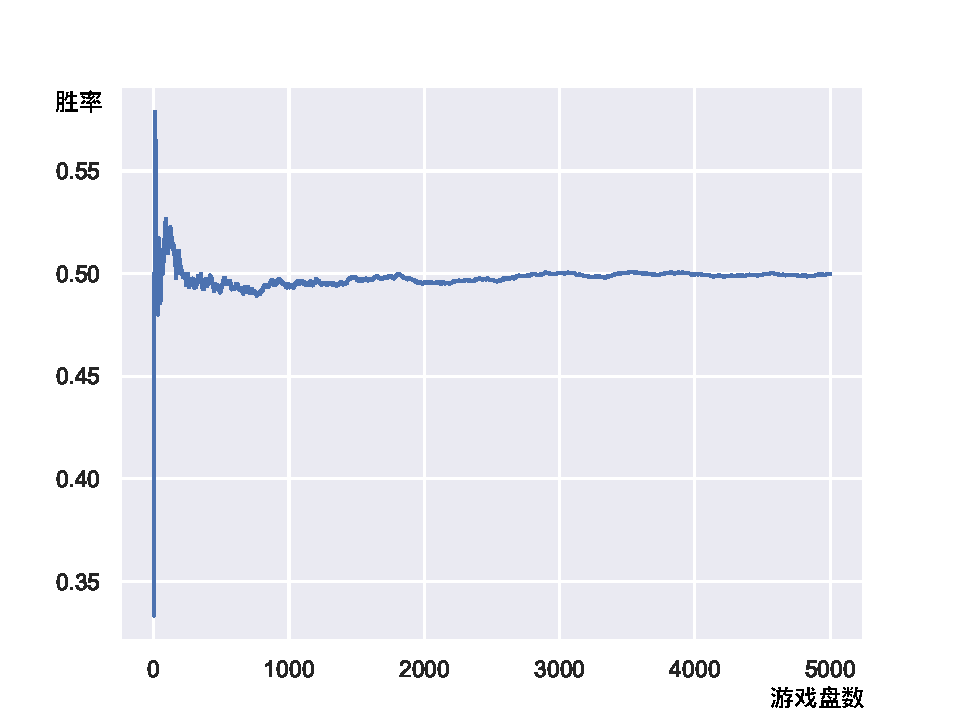
\includegraphics[width=12cm]{fair_game}
    \caption{对第五关博弈策略的重复实验}
    \label{fair_game}
\end{figure}

可以看到,随着游戏次数的增加,玩家1的资金比例收敛在50\%(相应地,玩家2的资金比例也如此收敛)。这说明,对于完全相同的若干玩家,无论其如何做出决策,只要他们做出决策的依据完全相同,其博弈的结果最终将达到完全的均衡。

因此,需要对不同的玩家引入不同的属性。面临博弈时,有些玩家不顾消耗数倍资源的风险,毅然选择继续前进,称为“风险偏好者”;有些玩家选择小心谨慎,宁可绕路也不想遭遇冲突带来额外的资源耗费,称为“风险厌恶者”。不同的玩家具有不同的风险接受程度,这就使得他们做出决策的依据有所区别,对博弈结果的讨论将更有意义。

\textbf{(3)状态转移概率}

为了刻画玩家考虑当前状态并做出决策的过程,即在$ \ s_k $的状态做出某动作的概率,引入风险接受程度作为状态转移概率
\begin{equation}
    T(\ S,\ a,S\prime\ )\ \sim P_r(\ s\prime\ |\ s,\ a)
\end{equation}
多个玩家的最优路径出现冲突时,如果某一玩家的最优路径也是唯一可行路径,那他将别无所选。除此之外,不同风险偏好的玩家的状态转移概率有所差别,如表\ref{tab:p6RiskPreference}所示。

\begin{table}[!htbp]
    \caption{不同风险偏好的状态转移概率差别}\label{tab:p6RiskPreference} 
    \centering
    \begin{tabular}{cc}
        \toprule[1.5pt]
        风险偏好 & 对状态转移概率的影响 \\
        \midrule[1pt]
        风险偏好者 & 玩家以$66.6\%-100\%$的概率往冲突点移动\\
        风险中性者 & 玩家以$33.3\%-66.6\%$的概率往冲突点移动 \\
        风险厌恶者 & 玩家以$0\%-33.3\%$的概率往冲突点移动 \\
        \bottomrule[1.5pt]
    \end{tabular}
\end{table}

\textbf{(4)回报}

当发生了状态转移,这一动作会带来回报,一步动作的收益可被刻画为
\begin{equation}
R(\ S,\ a\ )\ =\ E[R_{t+1}\ |\ s,\ a\ ]
\end{equation}
过程的目标函数是所有状态的和最大,考虑游戏时间为30天,故将本问模型目标函数表示为:
\begin{equation}
\ max\ U(s_0,\ s_1,\ ...,s_{30})\ =\ \sum_{t=0}^{30}{R(s_t,\ a_t)\ }
\end{equation}

\subsubsection{模型求解}
使用\textbf{蒙特卡洛模拟}方法构建仿真程序,模拟不同风险接受程度的玩家的马尔可夫决策过程,进而探究风险接受程度的高低对玩家做出决策优劣的影响。

每一次模拟中,所有玩家除风险接受程度(状态转移概率)外的的初始条件完全相同,每位玩家的风险接受程度由程序随机指定。每一阶段,玩家考虑其他玩家的可能行动方向与自身从当前位置到终点的最优子策略是否存在冲突,若冲突则依据风险接受程度做出前往冲突点或绕路的决策。仿真过程中最优子策略的求解方法与问题一中的动态规划求解方法相同。每一次模拟结束后,记录每位玩家的决策路径、最终剩余资金。若玩家由于资源或资金不足导致未能到达终点(游戏失败),则最终剩余资金为0。

对仿真结果进行分析,最终剩余资金最多的玩家中,同时也是当局游戏三位玩家中风险接受程度最高的玩家的比例约为40\%(占比最高),这些玩家中,多数都是风险偏好者和风险厌恶者。然而,仿真结果也显示,过高的风险接受程度带来的过多冲突将消耗过多资源,导致游戏失败。为了探究合适的风险接受程度,对所有游戏失败玩家的风险接受程度进行统计,可绘制直方图并进行核密度估计,结果如图\ref{kde}所示。

\begin{figure}[!h]
    \centering
    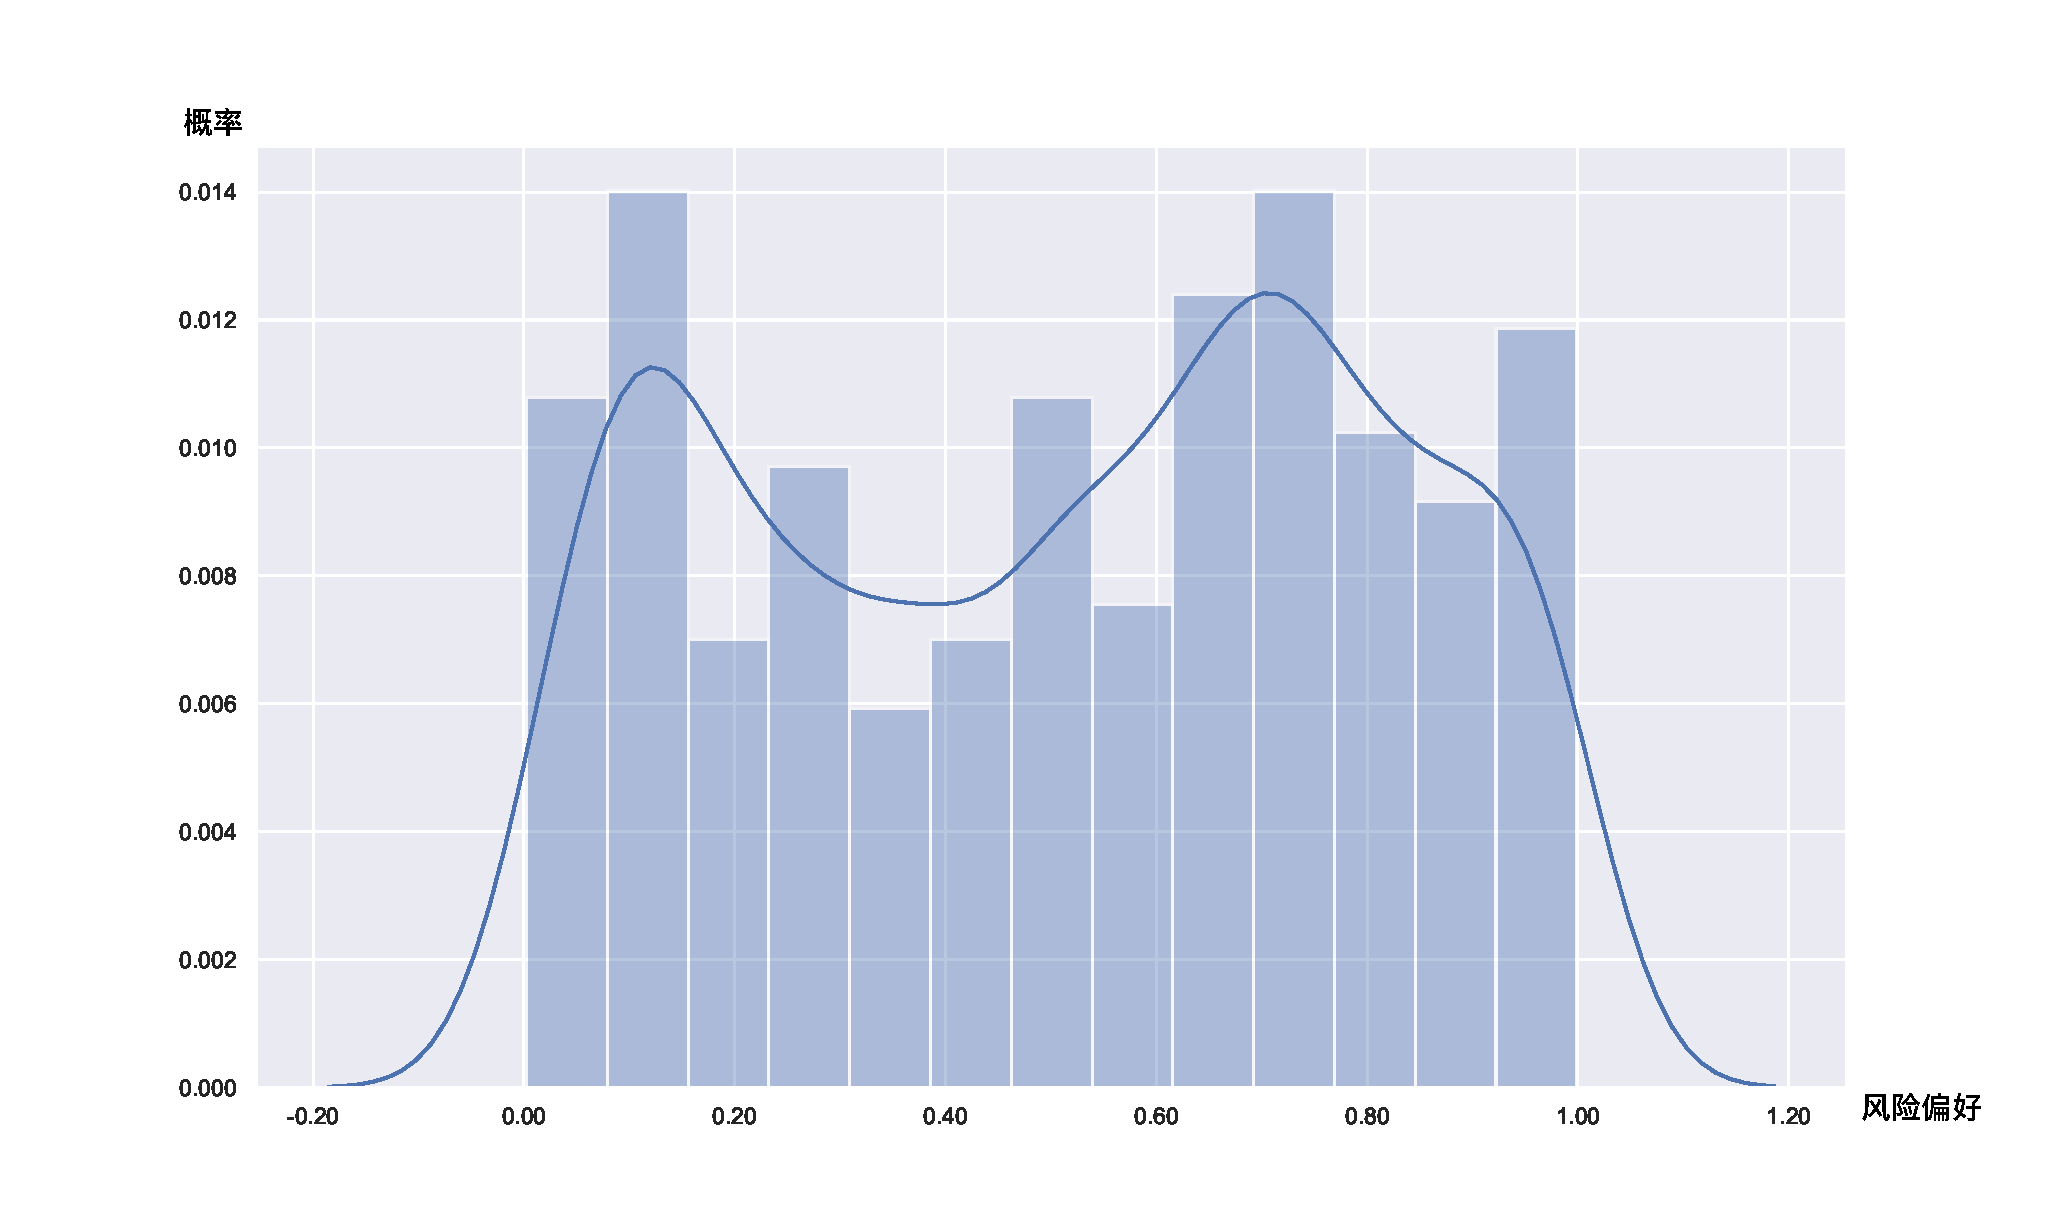
\includegraphics[width=12cm]{kde}
    \caption{所有游戏失败玩家的风险接受程度的核密度估计}
    \label{kde}
\end{figure}

可以看出,风险接受程度在20\%至60\%的玩家游戏失败的可能性较低。结合风险接受程度与最终剩余资金的关系,保持60\%左右的风险接受程度是一个好的策略。

\section{模型评价与推广}
\label{sec:simulate}

\subsection{问题一}

对于问题一,将原始地图简化为有向图模型后,通过分析游戏规则中的决策方案和约束条件,建立了完整的动态规划模型,包括状态变量、决策变量、状态转移函数、损益函数等。在算法实现中,结合多重搜索、记忆化搜索、剪枝等优化手段,显著提升了计算速度。

基于该模型和算法,可以直接求解出第一、二关的全局最优策略。模型的适应性强、稳定性高,在只有一名玩家的条件下,模型可以推广到任意一种全程天气状况已知的地图情形。

\subsection{问题二}

在环境不确定的情况下,该模型通过分析不确定因素的累计情况,通过调整Dijkstra算法,创建了以关键位置为核心的简化网络,并以此为基础建立了玩家的决策路径。
同时,也建立了玩家的收益与各个行为之间的关联,从而建立了数个基础的决策依据,具体环境下,只需进行成本分析和环境分析,即可获得玩家的一般最佳策略。

第三关与第四关的条件类似,由于关键结点之前玩家碰到的环境不一致,在关键结点玩家需要根据具体的情况做出决策,同时计算出玩家在不同情况下的收益,考虑
环境的不确定性,即可分析出最佳策略,该模型可以推广到其他问题。


\subsection{问题三}

对于问题三,基于静态博弈与动态博弈的思路,在多玩家参与且决策结果会互相影响的情况下,基于前两问的部分结论,建立了玩家的行为策略的基本模型。

对于第五关的静态完全信息博弈,假定了玩家之间不存在任何信息交换。模型抽象出三种决策选择,从混合策略的角
度计算策略的概率能够从大数量盘数的游戏中保证金额均值的最大化,但是对于一局游戏的决策的指导意义有限。

对于第六关,引入风险偏好对玩家在博弈中的选择倾向进行刻画,这一点适应了实际游戏玩家并非完全理性人的实际情况。在模型的求解上,扩展了问题一
的模型,用动态规划求解马尔可夫决策过程的结果最大化问题,比较好地还原了游戏规则中的决策情况。但模型没有考虑玩家间利用规则开展合作、报复等操作,在人为因素的刻画上仍可改善。



%参考文献
\begin{thebibliography}{9}%宽度9
    \bibitem[1]{book:OR}
    沈荣芳.
    \newblock 运筹学\allowbreak[M].
    \newblock 机械工业出版社, 北京, 2015.
    \bibitem[2]{linear}
    Luenberger D G, Ye Y.
    \newblock Linear and nonlinear programming\allowbreak[M].
    \newblock Reading, MA: Addison-wesley, 1984.
    \bibitem[3]{algorithm}
    Cormen T H, Leiserson C E, Rivest R L, et al.
    \newblock Introduction to algorithms\allowbreak[M].
    \newblock MIT press, 2009.
    \bibitem[4]{game}
    Osborne M J, Rubinstein A.  
    \newblock A course in game theory.\allowbreak[M].
    \newblock MIT press, 1994.
\end{thebibliography}


















\newpage

\newpage
%附录
\begin{appendices}

\section{第一关结果}
    
\begin{figure}[!h]
    \centering
    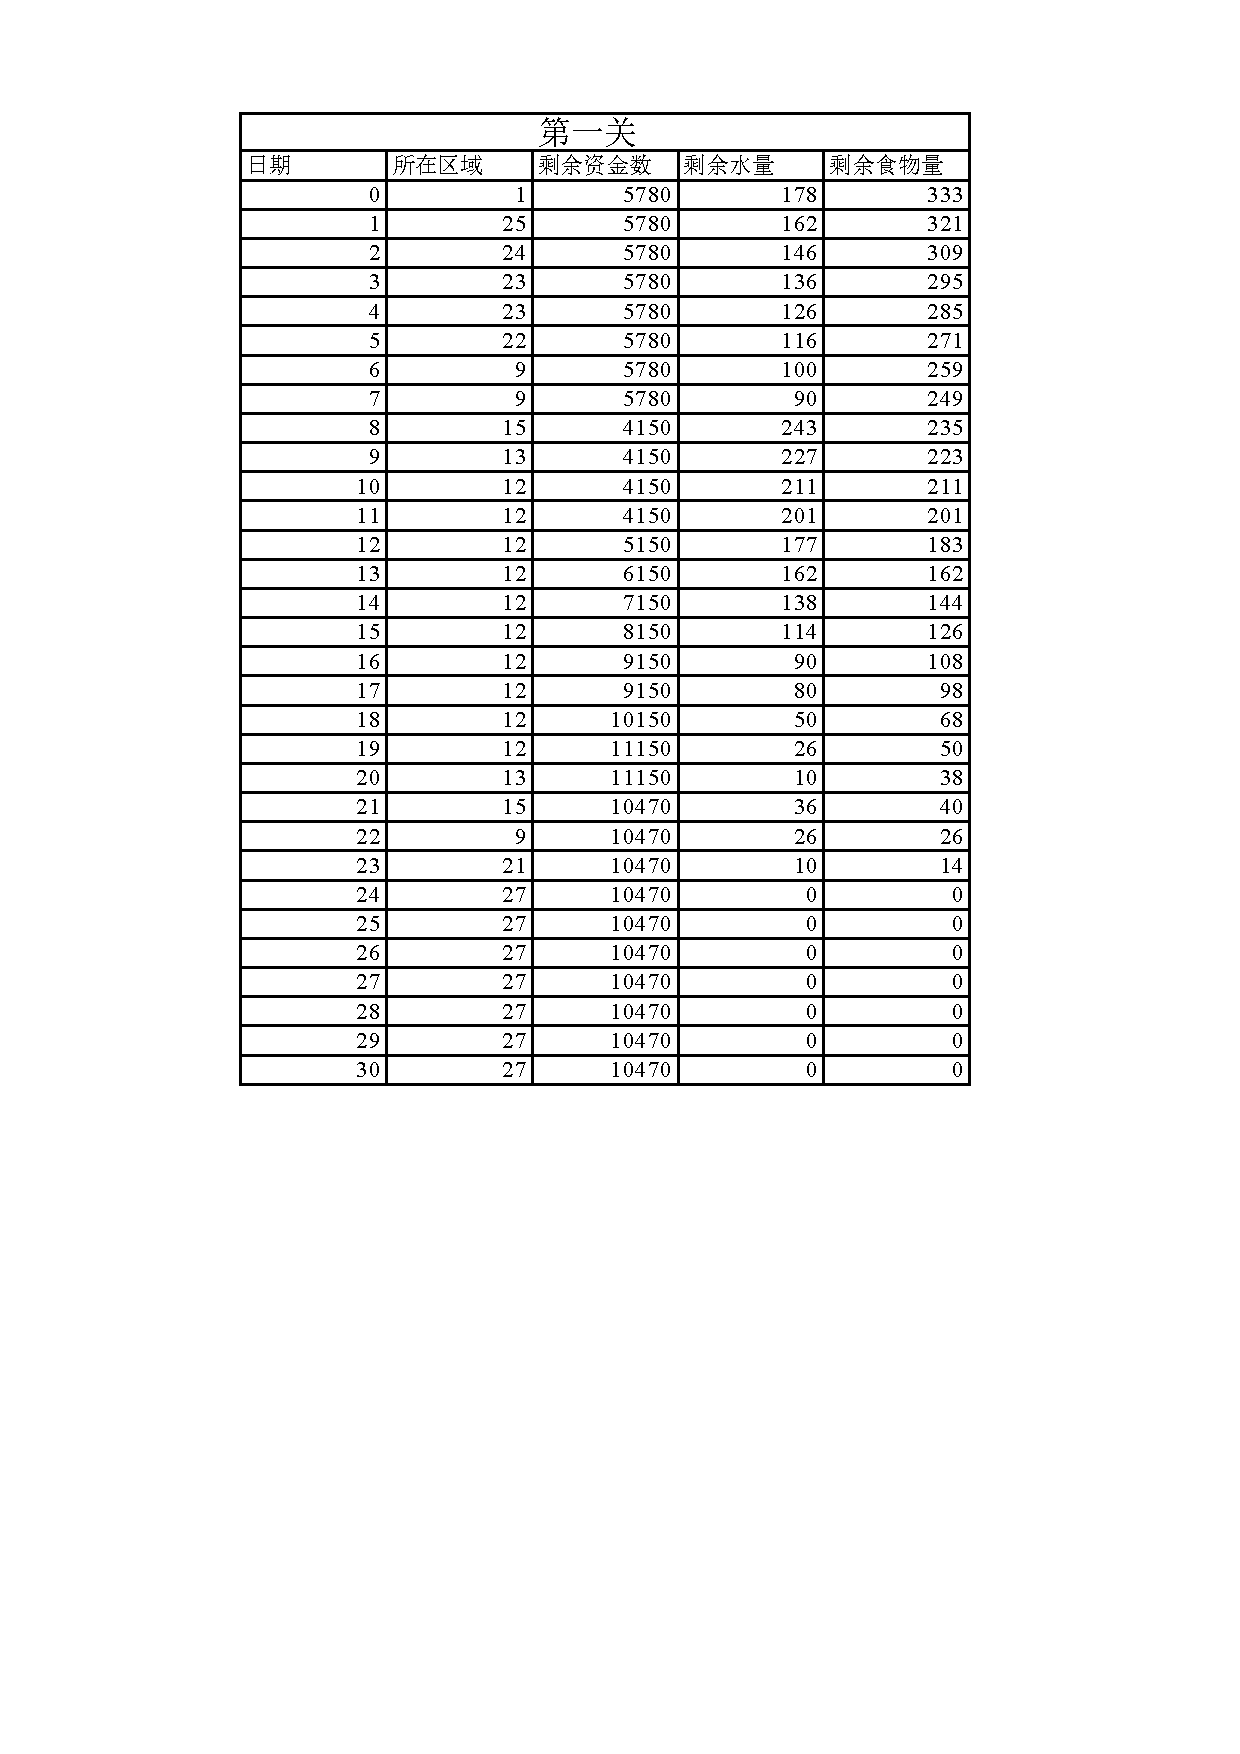
\includegraphics[width=.99\textwidth]{result1}
    \label{fig:result1}
\end{figure}
    
\newpage

\section{第二关结果}
    
\begin{figure}[!h]
    \centering
    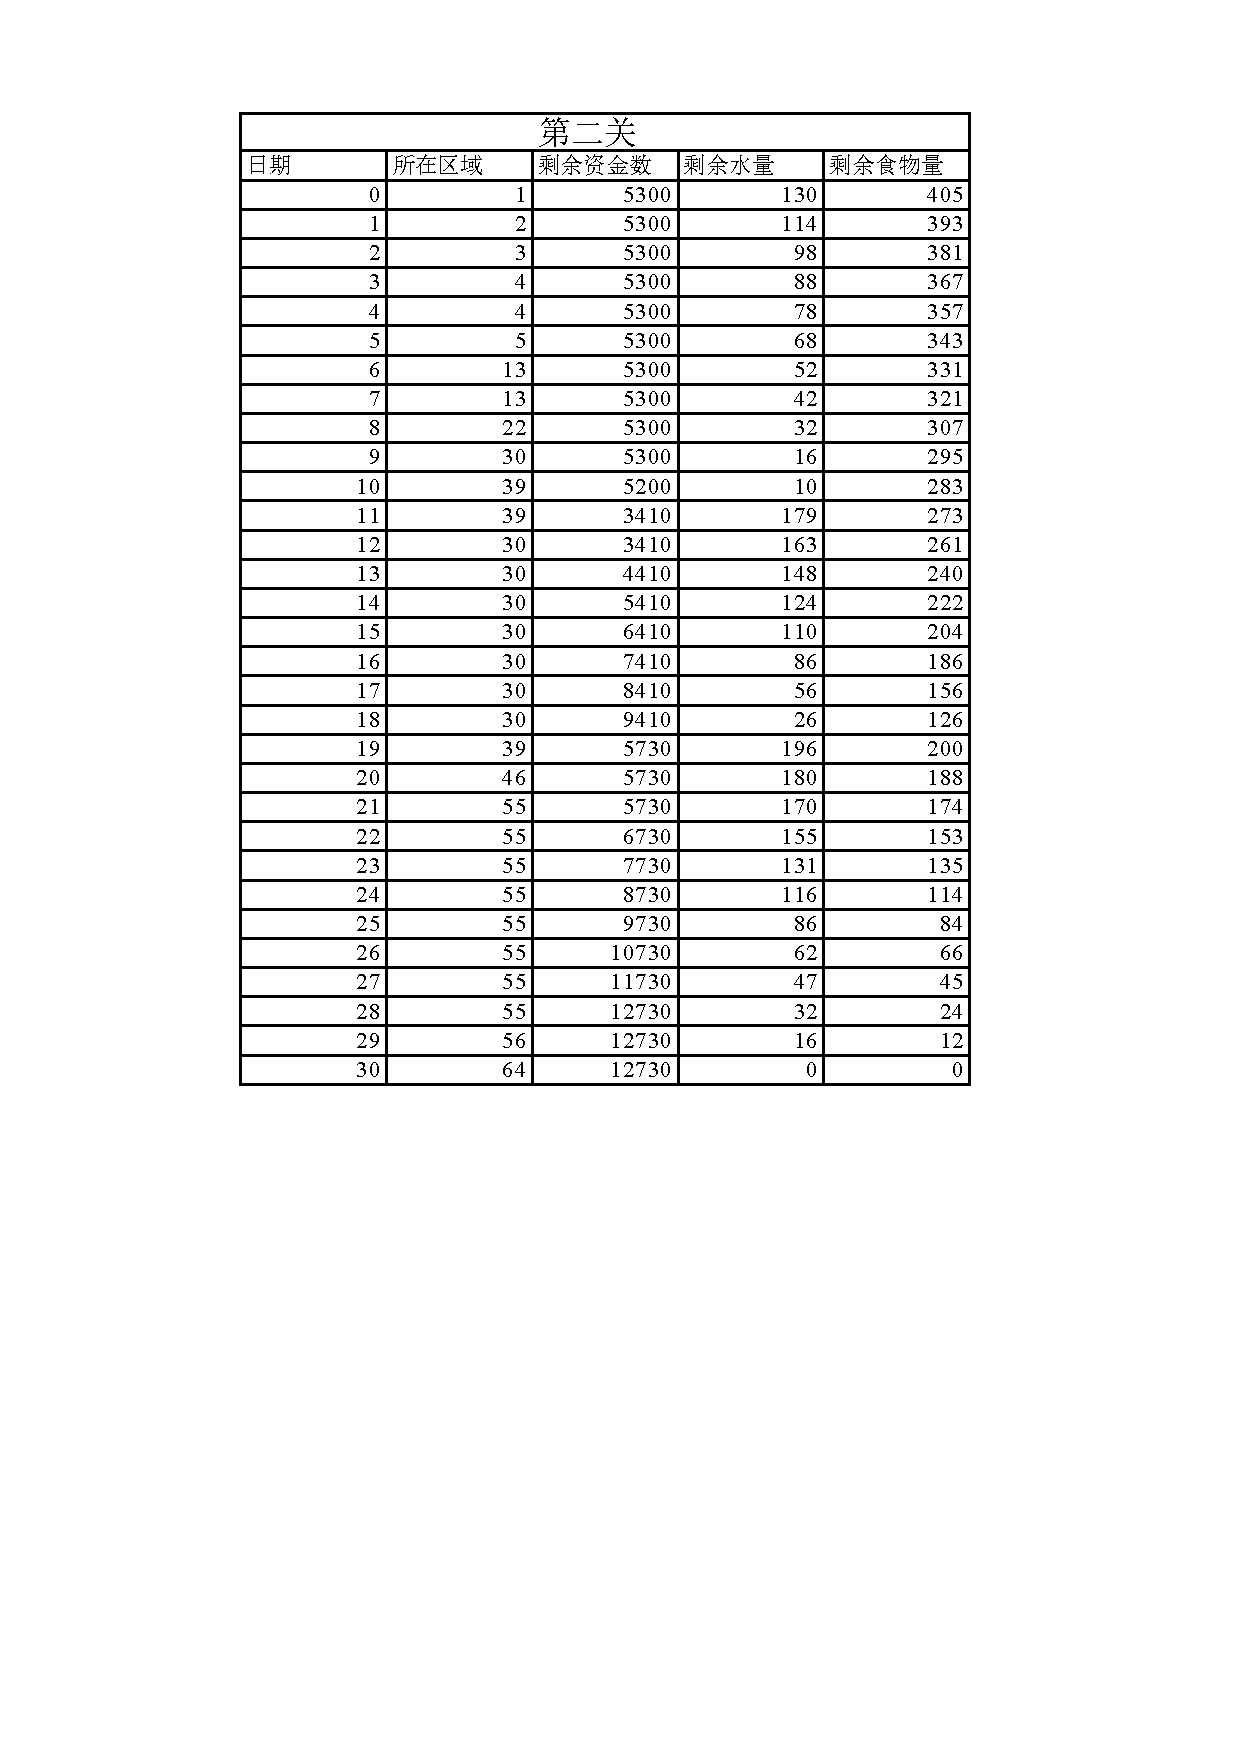
\includegraphics[width=.99\textwidth]{result2}
    \label{fig:result2}
\end{figure}
    
\newpage

\section{最短路径源码}

\begin{lstlisting}
'''
算法说明:getAllRoutes基于对最路径算法Dijkstra算法修改,实现获得两点之
间最短路径的功能;getKeyPoint则是文中提到的寻找可能会做出决策关键位置,
是路径交点中,离两个点最近的位置。该算法可以实现模型的简化,也可以寻找潜在
产生决策的位置。
    
案例说明:第三关中,寻找起点1号到矿山9号和终点13号的可能关键结点,首先计算
出起点到达矿山和终点的全部最短路径,计算其公共位置,从公共位置中选择出到矿
山和终点的距离之和最短的位置,该位置4号即为可能产生决策的位置。
'''
import pandas as pd
import json
import copy
    
# 获得路径的全部交点,选择离目标位置最近的点
def getKeyPoint(routes1, routes2, pt1, pt2):
    all_inters = getAllInters(routes1,routes2)
    min_distance = 99999999
    key_pt = []
    for inter in all_inters:
        routes1 = getAllRoutes(inter,pt1)
        routes2 = getAllRoutes(inter,pt2)
        distance = len(routes1[0]) + len(routes2[0])
        if distance < min_distance:
            key_pt = inter
            min_distance = distance
    return key_pt
        
# 获得两个最短路径的可能交点
def getAllInters(routes1,routes2):
    all_inters = []
    for route1 in routes1:
        for route2 in routes2:
            for i in range(1,len(route1)):
                if route1[i] in route2:
                    all_inters.append(route1[i])
    return all_inters
    
# 根据有向链求解全部的途径
def getAllRoutes(from_id, to_id):
    front_neighbors = getAllFrontNeighbor(from_id, to_id)
    routes = []
    reversed_routes = [[to_id]]
    temp_reversed_routes = []
    i = 0
    while True:
        get_end = False
        temp_reversed_routes = []
        for route in reversed_routes:
            for front_pt in front_neighbors[route[-1]-1]:
                temp_reversed_routes.append(route+[front_pt]) # 仅仅append处理是不增加的!!!
                if front_pt == from_id:
                    get_end = True
        reversed_routes = copy.deepcopy(temp_reversed_routes)
        if get_end == True:
            break
        i = i +1 
    for item in reversed_routes:
        item.reverse()
        routes.append(item)
    return routes
    
# 获得全部的单向网络
def getAllFrontNeighbor(from_id,to_id):
    cur_pts = [from_id] # 当前本轮外面的点
    searched_pts = [from_id] # 已经检索过的位置
    around_graph = [] # 按照距离存储的图
    cur_distance = 1 # 当前距离
    front_neighbors = [[] for i in range(problem.shape[0])] # 前面的邻接边,可能有多条
    
    while True:
        # 首先计算出全部的周边点
        all_neighbor_pts = []
        for cur_pt in cur_pts:
            for pt_id in neighbors[cur_pt-1]:
                if pt_id not in searched_pts:
                    if pt_id not in all_neighbor_pts:
                        all_neighbor_pts.append(pt_id)
                    front_neighbors[pt_id-1].append(cur_pt)
        # 计算完该轮区域
        around_graph.append(all_neighbor_pts)
        cur_pts = all_neighbor_pts
        searched_pts = searched_pts + all_neighbor_pts
    
        if to_id in searched_pts:
            break
    
    return front_neighbors
    
if __name__ == "__main__":
    problem_id = 3
    problem = pd.read_csv("problem/problem" + str(problem_id) + "_graph.csv")
    neighbors = []
    
    for i in range(problem.shape[0]):
        neighbors.append(json.loads(problem["neighbor"][i]))
    
    from_id, to_id1 = 1, 13 # 起始位置与目标位置
    routes1 = getAllRoutes(from_id,to_id1) # 获得全部的路径
    print("1-13的全部路径:")
    print(routes1)
        
    from_id, to_id2 = 1, 9 # 起始位置与目标位置
    routes2 = getAllRoutes(from_id,to_id2) # 获得全部的路径
    print("1-9的全部路径:")
    print(routes2)
    
    key_pt = getKeyPoint(routes1,routes2,to_id1,to_id2)
    print("起点前往终点和矿山的潜在决策位置:")
    print(key_pt)
    
\end{lstlisting}


\newpage


\section{动态规划源码}
    
\begin{lstlisting}
    from random import random,choice,shuffle

    class Point:
        def __init__(self,index):
            self.name=index
            self.neighbours=[]
            self.type=0
            self.players=0
            # 0 1 2 3 4: 普通 村庄 矿山 起点 终点
    
        def addNeighbour(self,pt):
            self.neighbours.append(pt)
    
        def setType(self,t):
            self.type=t
    
    class Solution:
        def __init__(self,step,prev,money,pt,key):
            self.step=step
            self.prev=prev
            self.next=[]
            self.money=money
            self.pt_index=pt
            self.key=key
            self.last_supply=key
            self.last_supply_pt=0
            self.last_cash=money
    
    class Decision:
        def __init__(self,start,end,weather,getMineral=False):
            self.start,self.end,self.weather=start,end,weather
            self.water=self.food=self.money=0 # 消耗为正 赚得为负 水或食物单位为箱
            if start.name==end.name and start.type!=4:
                if getMineral:
                    self.getMineral(weather)
                else:
                    self.water=WATER_CONSUMPTION[weather]
                    self.food=FOOD_CONSUMPTION[weather]
            if start.name!=end.name:
                self.water=2*WATER_CONSUMPTION[weather]
                self.food=2*FOOD_CONSUMPTION[weather]
                if MOVE_PLAN[start.name-1][end.name-1]>1:
                    self.water=self.water*MOVE_PLAN[start.name-1][end.name-1]
                    self.food=self.food*MOVE_PLAN[start.name-1][end.name-1]
    
    
        def getMineral(self,weather):
            self.water=3*WATER_CONSUMPTION[weather]
            self.food=3*FOOD_CONSUMPTION[weather]
            if POINTS[self.start.name-1].players>1:
                if MINING>0:
                    self.money=-PROFIT/MINING
                else:
                    self.money=-PROFIT
            else:
                self.money=-PROFIT
    
    WEATHER=[]
    DAY_NUM=0
    MAX_BURDEN=0
    INIT_MONRY=0
    PROFIT=0
    WATER_WEIGHT=0
    WATER_PRICE=0
    FOOD_WEIGHT=0
    FOOD_PRICE=0
    WATER_CONSUMPTION={}
    FOOD_CONSUMPTION={}
    POINTS=[]
    POINT_NUM=0
    DESTINATION=0
    MOVE_PLAN=[]
    MINING=0
    WATER_ADD={}
    FOOD_ADD={}
    MONEY_REDUCE={}
    
    def loadPoints(file_name):
        with open(file_name, 'r') as f:
            for line in f.readlines():
                line=line.split(',')
                p=Point(int(line[0]))
                POINTS[int(line[0])-1]=p
                if line[2].replace('\n','')!='':
                    p.setType(int(line[2]))
        with open(file_name, 'r') as f:
            for line in f.readlines():
                line=line.split(',')
                if line[1]!='':
                    for pt in line[1].split(' '):
                        POINTS[int(line[0])-1].addNeighbour(POINTS[int(pt)-1])
    
    def loadEnvir(problem_no):
        global WEATHER
        global DAY_NUM
        global MAX_BURDEN
        global INIT_MONRY
        global PROFIT
        global WATER_WEIGHT
        global WATER_PRICE
        global FOOD_WEIGHT
        global FOOD_PRICE
        global WATER_CONSUMPTION
        global FOOD_CONSUMPTION
        global POINT_NUM
        global DESTINATION
        global MOVE_PLAN
        if problem_no==1 or problem_no==2:
            WEATHER='高温,高温,晴朗,沙暴,晴朗,高温,沙暴,晴朗,高温,高温, \
                沙暴,高温,晴朗,高温,高温,高温,沙暴,沙暴,高温,高温,晴朗,晴朗, \
                高温,晴朗,沙暴,高温,晴朗,晴朗,高温,高温'.split(',') 
            DAY_NUM=30
            MAX_BURDEN=1200
            INIT_MONRY=10000
            PROFIT=1000
            WATER_WEIGHT=3
            WATER_PRICE=5
            FOOD_WEIGHT=2
            FOOD_PRICE=10
            WATER_CONSUMPTION={'晴朗':5,'高温':8,'沙暴':10}
            FOOD_CONSUMPTION={'晴朗':7,'高温':6,'沙暴':10}
            POINT_NUM=12 if problem_no==1 else 17
            DESTINATION=9 if problem_no==1 else 12
            assert(len(WEATHER)==DAY_NUM)
            for i in range(POINT_NUM):
                POINTS.append([])
                MOVE_PLAN.append([])
                for j in range(POINT_NUM):
                    MOVE_PLAN[i].append(0)            
            loadPoints('problem/problem{}_graph_simple.csv'.format(problem_no))
        if problem_no==6:
            DAY_NUM=30
            MAX_BURDEN=1200
            INIT_MONRY=10000
            PROFIT=1000
            WATER_WEIGHT=3
            WATER_PRICE=5
            FOOD_WEIGHT=2
            FOOD_PRICE=10
            WATER_CONSUMPTION={'晴朗':3,'高温':9,'沙暴':10}
            FOOD_CONSUMPTION={'晴朗':4,'高温':9,'沙暴':10}
            POINT_NUM=25
            DESTINATION=24
            for i in range(POINT_NUM):
                POINTS.append([])
                MOVE_PLAN.append([])
                for j in range(POINT_NUM):
                    MOVE_PLAN[i].append(0)  
            loadPoints('problem/problem6_graph.csv') 
    
    def getDecision(point,day):
        decision_list=[]
        if WEATHER[day]!='沙暴':
            for pt in point.neighbours:
                decision_list.append(Decision(point,pt,WEATHER[day]))
        decision_list.append(Decision(point,point,WEATHER[day]))
        if point.type==2:
            decision_list.append(Decision(point,point,WEATHER[day],getMineral=True))
        return decision_list
    
    def getKey(water,food):
        return str(water).zfill(4)+str(food).zfill(4)
    
    def revertKey(key):
        return int(key[0:4]),int(key[4:8])
    
    def dp_main(init_water,init_food,start_day=0,init_pt=0,init_money=None,\
            all_path=False):
        global WATER_ADD
        global FOOD_ADD
        global MONEY_REDUCE
        solution=[]
        for i in range(DAY_NUM+1):
            solution.append([])
            for j in range(POINT_NUM):
                solution[i].append({})            
        cur_key=getKey(init_water,init_food)
        if init_money==None:
            init_m=INIT_MONRY-init_water*WATER_PRICE-init_food*FOOD_PRICE
        else:
            init_m=init_money
        solution[start_day][init_pt][cur_key]=Solution(start_day,None,init_m, \
            init_pt, cur_key)
        for step in range(start_day,DAY_NUM):
            real_date=step # 顺序法
            pt_list=list(range(POINT_NUM))
            shuffle(pt_list)
            for pt in pt_list:
                records=solution[step][pt]
                if len(records)==0:
                    continue                   
                decisions=getDecision(POINTS[pt],real_date)
                shuffle(decisions)
                for d in decisions:
                    _water,_food,_money=d.water,d.food,d.money #变化量
                    for key in list(records.keys()):
                        cur_solution=records[key]
                        # if key=='00140228' and step==9 and pt==16:
                        #     print(9)
                        water,food=revertKey(key)
                        new_water=water-_water
                        new_food=food-_food
                        new_money=cur_solution.money-_money
                        last_cash=cur_solution.last_cash
                        last_supply=cur_solution.last_supply
                        last_supply_pt=cur_solution.last_supply_pt
                        if d.end.type==4 or d.end.type==1:
                            last_water,last_food=revertKey(last_supply)
                            last_cash=new_money
                            water_buy,food_buy=0,0
                            if new_water<0:
                                water_buy=-new_water
                            if new_food<0:
                                food_buy=-new_food
                            if water_buy>0 or food_buy>0:
                                if last_supply==cur_key:
                                    continue
                                canBuy=False
                                if POINTS[last_supply_pt].players<2:
                                    cost_k=2
                                if POINTS[last_supply_pt].players>1:
                                    cost_k=4
                                cost=water_buy*WATER_PRICE*cost_k+food_buy*\
                                    FOOD_PRICE*cost_k
                                if (last_water+water_buy)*WATER_WEIGHT+(last_food+ \
                                        food_buy)*FOOD_WEIGHT<=MAX_BURDEN and cost<=last_cash:
                                    canBuy=True
                                if canBuy:
                                    new_money=new_money-cost
                                    new_water=new_water+water_buy
                                    new_food=new_food+food_buy
                                    WATER_ADD[last_supply]=water_buy
                                    FOOD_ADD[last_supply]=food_buy
                                    MONEY_REDUCE[last_supply]=cost
                                    last_cash=new_money
                                    last_supply=getKey(new_water,new_food)
                                    last_supply_pt=d.end.name-1
                                else:
                                    continue
                            else:
                                last_supply=getKey(new_water,new_food)
                                last_supply_pt=d.end.name-1
                        new_key=getKey(new_water,new_food)   
                        new_solution=Solution(step+1,cur_solution,new_money, \
                            d.end.name-1,new_key)
                        new_solution.last_cash=last_cash
                        new_solution.last_supply=last_supply
                        new_solution.last_supply_pt=last_supply_pt
                        cur_solution.next.append(new_solution)
                        if new_key in solution[step+1][d.end.name-1]:
                            if solution[step+1][d.end.name-1][new_key].money> \
                                    new_solution.money:
                                continue
                        solution[step+1][d.end.name-1][new_key]=new_solution
        final=solution[DAY_NUM][DESTINATION]
        final_pts=[]
        final_pt=None
        max_finals=[]
        max_final=0
        for key in final:
            water,food=revertKey(key)
            if water<0 or food<0:
                continue
            max_finals.append(water*WATER_PRICE*0.5+food*FOOD_PRICE*0.5+ \
                final[key].money)
            final_pts.append(final[key])
        for index,value in enumerate(max_finals):
            if value>=max_final:
                max_final=value
                final_pt=final_pts[index]
        with open('output.csv','a') as f:
            f.write(str([init_water,init_food,max_final]) \
                .replace('[','').replace(']','')+'\n')
        if not all_path:
            return final_pt,max_final
        else:
            return final_pt,max_final,final_pts,max_finals
    
    def dp_all(problem_no):
        # 多重搜索+动态规划 求解第一关和第二关
        loadEnvir(problem_no)
        global_max=0
        final_pt=None
        max_ij=[0,0]
        for p in range(0,int(MAX_BURDEN/WATER_WEIGHT)):
            for q in range(0,int(MAX_BURDEN/FOOD_WEIGHT)):
                if p*WATER_WEIGHT+q*FOOD_WEIGHT>MAX_BURDEN:
                    continue
                final,max_final=dp_main(p,q)
                if max_final>global_max:
                    global_max=max_final
                    final_pt=final
                    max_ij=[p,q]
        while final_pt!=None:
            print(final_pt.step,final_pt.pt_index,final_pt.money,final_pt.key)
            final_pt=final_pt.prev
        print(max_ij,global_max)
    
    def dp_game(risk):
        # 多重静态博弈 求解第六关
        water=[200,200,200]
        food=[300,300,300]
        player_pt=[0,0,0]
        money=[6000,6000,6000]
        path=[[],[],[]]
        death=[False,False,False]
        global MINING
        global WATER_ADD
        global FOOD_ADD
        global MONEY_REDUCE
        global WEATHER
        for step in range(0,30):
            next_state=[None,None,None]
            MINING=0
            WATER_ADD,FOOD_ADD,MONEY_REDUCE={},{},{}
            for p in range(0,3):
                if death[p]:
                    continue
                final_pt,max_final=dp_main(water[p],food[p],step, \
                    player_pt[p],money[p])
                while final_pt!=None:
                    if final_pt.step==step+1:
                        next_state[p]=final_pt
                        break
                    final_pt=final_pt.prev
                if next_state[p]==None:
                    death[p]=True
                    money[p]=0
                    continue
                if next_state[p].money>money[p]:
                    MINING=MINING+1
            for i in range(POINT_NUM):
                POINTS[i].players=0
                for j in range(POINT_NUM):
                    MOVE_PLAN[i][j]=0
            for p in range(0,3):
                if death[p]:
                    continue
                next_pt_index=next_state[p].pt_index
                POINTS[next_pt_index].players=POINTS[next_pt_index].players+1
                MOVE_PLAN[player_pt[p]][next_pt_index]= \
                    MOVE_PLAN[player_pt[p]][next_pt_index]+1
            for p in range(0,3):
                if death[p]:
                    continue
                final_pt,max_final,final_pts,max_finals=dp_main(water[p],food[p], \
                    step,player_pt[p], money[p],all_path=True)
                best_plan,good_plan=None,None
                while final_pt!=None:
                    if final_pt.step==step+1:
                        best_plan=final_pt
                        break
                    final_pt=final_pt.prev
                if best_plan==None:
                    death[p]=True
                    money[p]=0
                    continue
                conflict=False
                for other in range(0,3):
                    if p==other:
                        continue
                    if death[other]:
                        continue
                    if best_plan.pt_index==next_state[other].pt_index:
                        conflict=True
                if  conflict:
                    if random()<risk[p]:
                        _water1,_food1=revertKey(best_plan.key)
                        _water2,_food2=revertKey(best_plan.prev.key)
                        water[p]=water[p]+_water1-_water2
                        food[p]=food[p]+_food1-_food2
                        if best_plan.pt_index in WATER_ADD:
                            water[p]=water[p]+WATER_ADD[best_plan.pt_index]
                        if best_plan.pt_index in FOOD_ADD:
                            food[p]=food[p]+FOOD_ADD[best_plan.pt_index]                    
                        money[p]=money[p]+best_plan.money-best_plan.prev.money
                        if best_plan.pt_index in MONEY_REDUCE:
                            money[p]=money[p]-MONEY_REDUCE[best_plan.pt_index]
                        player_pt[p]=best_plan.pt_index
                        path[p].append(best_plan.pt_index+1)
                    else:
                        good_max=0
                        for index,plan in enumerate(final_pts):
                            while plan!=None:
                                if plan.step==step+1:
                                    if plan.pt_index!=best_plan.pt_index:
                                        if max_finals[index]>good_max:
                                            good_max=max_finals[index]
                                            good_plan=plan
                                    break
                                plan=plan.prev
                        if good_plan==None:
                            good_plan=best_plan
                        _water1,_food1=revertKey(good_plan.key)
                        _water2,_food2=revertKey(good_plan.prev.key)
                        water[p]=water[p]+_water1-_water2
                        food[p]=food[p]+_food1-_food2
                        if good_plan.pt_index in WATER_ADD:
                            water[p]=water[p]+WATER_ADD[good_plan.pt_index]
                        if good_plan.pt_index in FOOD_ADD:
                            food[p]=food[p]+FOOD_ADD[good_plan.pt_index]
                        money[p]=money[p]+good_plan.money-good_plan.prev.money
                        if good_plan.pt_index in MONEY_REDUCE:
                            money[p]=money[p]-MONEY_REDUCE[good_plan.pt_index]
                        player_pt[p]=good_plan.pt_index
                        path[p].append(good_plan.pt_index+1)
                else:
                    _water1,_food1=revertKey(best_plan.key)
                    _water2,_food2=revertKey(best_plan.prev.key)
                    water[p]=water[p]+_water1-_water2
                    food[p]=food[p]+_food1-_food2
                    if best_plan.pt_index in WATER_ADD:
                        water[p]=water[p]+WATER_ADD[best_plan.pt_index]
                    if best_plan.pt_index in FOOD_ADD:
                        food[p]=food[p]+FOOD_ADD[best_plan.pt_index]
                    money[p]=money[p]+best_plan.money-best_plan.prev.money
                    if best_plan.pt_index in MONEY_REDUCE:
                        money[p]=money[p]-MONEY_REDUCE[best_plan.pt_index]
                    player_pt[p]=best_plan.pt_index
                    path[p].append(best_plan.pt_index+1)
            print(path,money)
        with open('game.csv','a') as f:
            f.write(str([risk[0],risk[1],risk[2],money[0],money[1],money[2]]) \
                .replace('[','').replace(']','')+'\n')
        with open('path.csv','a') as f:
            f.write(str(path)+'\n')
        with open('weather.csv','a') as f:
            f.write(str(WEATHER).replace('[','').replace(']','')+'\n')
    
    def dp_game_all():
        loadEnvir(6)
        global WEATHER
        global DAY_NUM
        for i in range(1000):
            WEATHER=[]
            for i in range(DAY_NUM):
                rd=random()
                if rd<0.1:
                    WEATHER.append('沙暴')
                elif rd<0.55:
                    WEATHER.append('晴朗')
                else:
                    WEATHER.append('高温')
            risk=[random(),random(),random()]
            print(risk)
            dp_game(risk)
    
    
    if __name__ == "__main__":
        dp_game_all() # 第六关求解
        # dp_all(2) # 第一关、第二关求解
                
\end{lstlisting}

\newpage



\section{求解混合策略Lingo源码}

\begin{lstlisting}
model:
sets:
k/1..3/:p;
n/1..3/:q;
pay(k,n):M;
endsets
data:
M=9070 9425 9325
  9535 8850 9325
  9535 9425 8515;
enddata
max=money;
@for(n(j):
  money<@sum(k(i):p(i)*m(i,j));
);
@sum(k:p)=1;
End

\end{lstlisting}


% \begin{table}[h]
%     \centering
%     \csvautotabular{data/problem3_graph.csv}
%     \caption{第三关数据}
% \end{table}    

% \begin{table}[h]
%     \centering
%     \csvautotabular{data/problem3_graph.csv}
%     \caption{第四关数据}
% \end{table} 





% \newpage

% \section{网络简化处理结果}


% \newpage

% \section{博弈仿真结果}


\end{appendices}

\end{document} 